%preamble - package inclusion and set up
%page setup (page size, text size, page layout, chapters start on a new page).
%memoir is a form of book class that supports any kind of document.
\documentclass[fleqn,a4paper,12pt,twoside,openany,danish]{memoir}

%setting the header and footer in that order:
\setheadfoot{28pt}{28pt} %if any problems are encountered, try changing the latter 28pt with 1cm.

%setting language:
\RequirePackage[danish]{babel}

\usepackage{tocbibind}

%this package makes it possible to treat any element as a float,
%figures and tables are by default treated as floats.
%read http://en.wikibooks.org/wiki/LaTeX/Floats,_Figures_and_Captions to specify your float.
\usepackage{float}
\usepackage{wrapfig}
\usepackage{placeins}
\usepackage{tabu}

%this package makes it possible to make theorems and examples:
\usepackage{amsthm}
%setting the style of examples (parameters: plain, definition, remark):
%(definition is usually used for examples)
\theoremstyle{definition}
%the frist parameter is the syntax used in the document, the second is that which is printed in LaTex.
\newtheorem{example}{Eksempel}

%making it possible to use æ, ø and å:
\usepackage[utf8]{inputenc}
%helps with word division when using æ, ø and å, and makes it ps-font rather than bmp:
\usepackage[T1]{fontenc}

%package for implementation of graphic files:
\usepackage{graphicx}

\usepackage{multirow}

%package for subfigures
%\usepackage{graphicx}
%\usepackage{caption}


%package for captions
\usepackage[nooneline,labelfont=bf]{caption}
%\usepackage{subcaption}

%%package for implementation of math:
\usepackage{amsmath , amsfonts , amssymb, float}

%allowing use of color:
\usepackage{color}
%allowing use of more colors also in tables (see: http://en.wikibooks.org/wiki/LaTeX/Colors):
\usepackage[usenames,dvipsnames,svgnames,table]{xcolor}

%hyperlinks in the tabel of contents - comment this out before the report is printed.
\usepackage{hyperref}
\hypersetup{
%	bookmarks = true,  % Show 'bookmark'-frame in pdf.
	colorlinks = true, % True = colored links, False = framed links.
	citecolor = black,  % Link color for references.
	linkcolor = black,  % Link color in table of contents.
	urlcolor = black,   % Link color for extern URLs.
}

%makes it possible to refer to the name of a chapter rather than just the number.
\usepackage{nameref}

%package for the SI unit standard
\usepackage{siunitx}
\usepackage{units}

%package for writing program code in latex
\usepackage{listings}

\lstset{ 
language=C,               	 	% choose the language of the code
basicstyle=\footnotesize,       % the size of the fonts that are used for the code
numbers=left,                   % where to put the line-numbers
numberstyle=\footnotesize,      % the size of the fonts that are used for the line-numbers
stepnumber=1,                   % the step between two line-numbers. If it is 1 each line will be numbered
numbersep=5pt,                  % how far the line-numbers are from the code
backgroundcolor=\color{white},  % choose the background color. You must add \usepackage{color}
showspaces=false,               % show spaces adding particular underscores
showstringspaces=false,         % underline spaces within strings
showtabs=false,                 % show tabs within strings adding particular underscores
frame=single,           		% adds a frame around the code
tabsize=2,          			% sets default tabsize to 2 spaces
captionpos=b,           		% sets the caption-position to bottom
breaklines=true,       			% sets automatic line breaking
breakatwhitespace=false,    	% sets if automatic breaks should only happen at whitespace
escapeinside={\%*}{*)}          % if you want to add a comment within your code
}

%setting references (using numbers) and supporting i.a. Chicargo-style:
\usepackage{etex}
\usepackage{etoolbox}
\usepackage{keyval}
\usepackage{ifthen}
\usepackage{url}
\usepackage{csquotes}
\usepackage[backend=biber,url=true,doi=true,style=numeric, sorting=none]{biblatex}
\bibliography{bibliography/bibliography.bib}


%this package makes it possible include pdf pages in fx appendix;
%using  following syntax: \includepdf[pages={1}]{myfile.pdf}
\usepackage{pdfpages}

%%%MARGINER%%%
\setlrmarginsandblock{3.5cm}{2.5cm}{*}	% \setlrmarginsandblock{inner margin}{outer margin}{ratio}
\setulmarginsandblock{2.5cm}{3.0cm}{*}	% \setulmarginsandblock{top}{bottom}{ratio}
\checkandfixthelayout 			            % fixes stuff..

%%%%% Afsnitsformatering %%%%%%
\setlength{\parindent}{6mm}				% Stoerrelsen af indryk
\setlength{\parskip}{0mm}				% Afstand mellem afsnit ved 2xenter
\linespread{1,1}						% Linje afstand 

%Enables the use FiXme refferences. Syntax: \fxnote{...}
%With "final" in stead of "draft" an error will ocure for every FiXme
%under compilation.
\usepackage[footnote,final,english,silent,nomargin]{fixme}

\addto\captionsdanish{% Replace "english" with the language you use
	\renewcommand{\contentsname}%
	{Indholdsfortegnelse}%
}

%%%CHAPTERLAYOUT%%%
%setting the color of the chapter number
\definecolor{numbercolor}{gray}{0.7}
%Downloaded chapter-setup:
\newif\ifchapternonum
\makechapterstyle{jenor}{
  \renewcommand\printchaptername{}
  \renewcommand\printchapternum{}
  \renewcommand\printchapternonum{\chapternonumtrue}
  \renewcommand\chaptitlefont{\fontfamily{pbk}\fontseries{db}\fontshape{n}\fontsize{25}{35}\selectfont\raggedleft}
  \renewcommand\chapnumfont{\fontfamily{pbk}\fontseries{m}\fontshape{n}\fontsize{1in}{0in}\selectfont\color{numbercolor}}
  \renewcommand\printchaptertitle[1]{%
    \noindent
    \ifchapternonum
    \begin{tabularx}{\textwidth}{X}
    {\let\\\newline\chaptitlefont ##1\par} 
    \end{tabularx}
    \par\vskip-2.5mm\hrule
    \else
    \begin{tabularx}{\textwidth}{Xl}
    {\parbox[b]{\linewidth}{\chaptitlefont ##1}} & \raisebox{-15pt}{\chapnumfont \thechapter}
    \end{tabularx}
    \par\vskip2mm\hrule
    \fi
  }
}
%setting chapter style:
\chapterstyle{jenor}

\makepagestyle{AAU}							% Definerer sidehoved og sidefod udseende frem til ...
\makepsmarks{AAU}{%
	\createmark{chapter}{left}{shownumber}{}{. \ }
	\createmark{section}{right}{shownumber}{}{. \ }
	\createplainmark{toc}{both}{\contentsname}
	\createplainmark{lof}{both}{\listfigurename}
	\createplainmark{lot}{both}{\listtablename}
	\createplainmark{bib}{both}{\bibname}
	\createplainmark{index}{both}{\indexname}
	\createplainmark{glossary}{both}{\glossaryname}
}
\nouppercaseheads											% Ingen Caps oenskes

\makeevenhead{AAU}{}{}{\leftmark}				% Definerer lige siders sidehoved (\makeevenhead{Navn}{Venstre}{Center}{Hoejre})
\makeoddhead{AAU}{\rightmark}{}{Aalborg Universitet}		% Definerer ulige siders sidehoved (\makeoddhead{Navn}{Venstre}{Center}{Hoejre})
\makeevenfoot{AAU}{\thepage}{}{}							% Definerer lige siders sidefod (\makeevenfoot{Navn}{Venstre}{Center}{Hoejre})
\makeoddfoot{AAU}{}{}{\thepage}								% Definerer ulige siders sidefod (\makeoddfoot{Navn}{Venstre}{Center}{Hoejre})
\makeheadrule{AAU}{\textwidth}{0.5pt}						% Tilfoejer en streg under sidehovedets indhold
\makefootrule{AAU}{\textwidth}{0.5pt}{1mm}					% Tilfoejer en streg under sidefodens indhold

\copypagestyle{AAUchap}{AAU}								% Sidehoved for kapitelsider defineres som standardsider, men med blank sidehoved
\makeoddhead{AAUchap}{}{}{}
\makeevenhead{AAUchap}{}{}{}
\makeheadrule{AAUchap}{\textwidth}{0pt}
\aliaspagestyle{chapter}{AAUchap}							% Den ny style vaelges til at gaelde for chapters
% ... her

\pagestyle{AAU}												% Valg af sidehoved og sidefod

\usepackage{textpos}

%depth of numbered headlines (part/chapter/section/subsection):
\setsecnumdepth{subsection}
\maxsecnumdepth{subsection}
%depth of the table of contents:
\settocdepth{subsection}

% Makes sure LaTeX does not stretch the text at page break:
\raggedbottom


%macros - please read this file
%Macro for 'where'-enviroment was improved by Andrea and Niels :-)

%-----------UNITS-------------------------------------------
\newcommand{\unit}[1]{&& \left[\si{#1}\right]}
%
%\newcommand{\unit}[1]{[\si{#1}]}            %<<| Use these if you want equations to be
%\newcommand{\eq}[2]{&&\si{#1} &= \si{#2}&&} %<<| centered.. .. will appear scrambled
%                                            %  | from one equation to the next though..
%                                            %  | and does not work with long equations.. :/
%
%-----------------------------------------------------------

%-----------WHERE ENVIRONMENT-------------------------------
\newenvironment{where}{\leavevmode{\parindent=1em\indent} Where:\\}{}
\newcommand{\va}[3]
{
  \begin{tabular}{p{20pt} p{40pt} p{290pt} l}
    & { $#1$ } & { #2 } & \ifthenelse{\isempty{ #3 }}  {}  {[{\si{#3}}]} \\
  \end{tabular}\\
}
%-----------------------------------------------------------

%-----------TikZ SETTINGS-----------------------------------
\tikzset{
  block/.style    = {draw, thick, rectangle,
                     minimum height = 2.1em,
                     minimum width = 1.7em},
  sum/.style      = {draw, circle, inner sep=3pt} %<--Adder
}
%-----------------------------------------------------------


%-----------Fanzy reference SETTINGS------------------------
%Figure references:
\newcommand{\figref}[1]{figure \ref{#1}}

%Figure references after full stop/period:
\newcommand{\Figref}[1]{Figure \ref{#1}}

%Table references:
\newcommand{\tabref}[1]{table \ref{#1}}

%Table references after full stop/period:
\newcommand{\Tabref}[1]{Table \ref{#1}}

%Section references:
\newcommand{\secref}[1]{section \ref{#1}} % on page \pageref{#1}}

%Section references:
\newcommand{\Secref}[1]{Section \ref{#1}} % on page \pageref{#1}}

%Subsection references:
\renewcommand{\subref}[1]{section \ref{#1}} % on page \pageref{#1}}

%Subsection references:
\renewcommand{\Subref}[1]{Section \ref{#1}} % on page \pageref{#1}}

%Appendix references:
\newcommand{\appref}[1]{appendix \ref{#1}} % on page \pageref{#1}}

%Appendix references:
\newcommand{\Appref}[1]{Appendix \ref{#1}} % on page \pageref{#1}}

%chapter references: 
\newcommand{\chapref}[1]{chapter \ref{#1}} % on page \pageref{#1}}

%chapter references: 
\newcommand{\Chapref}[1]{Chapter \ref{#1}} % on page \pageref{#1}}

%Units:
%\newcommand{\unit}[1]{&& \left[\si{#1}\right]}

%Text:
\newcommand{\tx}[1]{\text{#1}}

%Equation references:
%1 equation:
\renewcommand{\eqref}[1]{equation (\ref{#1})}

%-----------------------------------------------------------





\begin{document}       % TIP: If you are using TeXstudio you can open
%\tableofcontents      %      the file by Ctrl+LeftClick on setup/macros.tex
%\pagebreak             %      If the file doesn't exist, you will be asked
					   %      weather or not you want to create it.
%\begin{center}
%	\vspace{5cm}
%	\Huge{Worksheets}
%\end{center}
%\clearpage

%||||||||||||||||||||||||||||||||||||||||||||||||||||||||||||||||
%|||||||                 Example Inputs                  ||||||||
%||||||||||||||||||||||||||||||||||||||||||||||||||||||||||||||||
%|||||||                                                 ||||||||
%			 \input{chapters/aFigureSample.tex}			 %|||||||
%			 \input{chapters/bTableSample.tex} 		     %|||||||
%			 \input{chapters/cEquationSample.tex}		 %|||||||
%			 \input{chapters/dTikzSample.tex}            %|||||||
%			 \input{chapters/eCodeSample.tex}            %|||||||
%|||||||                                                 ||||||||
%||||||||||||||||||||||||||||||||||||||||||||||||||||||||||||||||
%||||||||||||||||||||||||||||||||||||||||||||||||||||||||||||||||


%%% Prereport %%%
		\setlength\cftaftertoctitleskip{2pt}
		\setlength\cftafterloftitleskip{6pt}
		\setlength\cftafterlottitleskip{6pt}
%\selectlanguage{danish}
%\title{Testing the performance of linear regressors using inertial information combined with sEMG to minimize the limb position effect in proportional and simultaneous control of lower arm prosthetics.}

%%% Frontmatter Settings %%%
		\pagestyle{empty} %disable headers and footers
		\pagenumbering{roman} %use roman page numbering in the frontmatter I II...
%		\fancyfoot[RE,LO]{17gr7404} %page number on all pages
%		\fancyfoot[LE,RO]{\thepage}
%		\fancyhead[LE,LO,RE,RO]{}

%%% Introductory Formalities %%%
%\includepdf[pages={1}]{formalities/frontpage.pdf}
%			\clearpage
\thispagestyle{empty}

\begin{figure}[H]
	\raggedleft
	\includegraphics[width=0.2\textwidth]{figures/aaulogo-en.png}
\end{figure} 

\vspace{5 cm}

\begin{center}
	\begin{Huge}
		\textbf{Examining if Confidence Score Feedback During User Training Can Improve Users’ Ability in Controlling Upper Limb Prosthetics}\\
		\vspace{5 mm}
		2nd semester Masters, Biomedical Engineering \& Infomatics - Spring $2018$\\
		\vspace{3 mm}
	\end{Huge}
	{\Large Project group: $18$gr$8408$} \\
	\vspace{1cm}
	\large{Simon Bruun, Oliver Thomsen Damsgaard, Martin Alexander Garenfeld, Christian Korfitz Mortensen}
\end{center}
\vspace*{\fill}

\begin{center}
	\line(1,0){400}
\end{center}

%\newpage
%
%\large{\textbf{Project period:}\\
%P7, Autumn 2017\\
%01/08/2017 - 20/12/2017\\
%
%\textbf{Project group:}\\
%17gr7404\\} %\fxnote{Input group number}
%
%
%\begin{center}
%	\Large{\textbf{Collaborators:}\\
%		\vspace{1.5cm}
%	\rule{10cm}{1pt}\\
%	Irene Uriarte \\
%	
%	\rule{10cm}{1pt}\\
%	Martin Alexander Garenfeld \\
%	
%	\rule{10cm}{1pt}\\
%	Oliver Thomsen Damsgaard \\
%	
%	\rule{10cm}{1pt}\\
%	Simon Bruun \\}
%\end{center}
%
%
%
%\large{\textbf{Supervisors:}\\
%Strahinja Dosen \\
%Jakob Lund Dideriksen \\
%Lotte N.S. Andreasen Struijk} \\
%\\
\newpage
			% <--- the frontpage
%			\pagestyle{fancy}
%%\include{formalities/kolofon}
%			%\begin{document} 
\thispagestyle{empty}
\begin{titlepage}
\begin{nopagebreak}
{\samepage 

\begin{tabular}{r}
\parbox{\textwidth}{  \raisebox{-15mm}{\includegraphics[height=3cm]{figures/aaulogo-en.png}}
\hfill \hspace{2cm} \parbox{8cm}{\begin{tabular}{l} %4.90
{\small \textbf{\textcolor{aaublue}{{7\textsuperscript{th} Semester, Masters Project}}}}\\
{\small \textbf{\textcolor{aaublue}{School of Medicine and Health}}}\\
%{\small \textbf{\textcolor{aaublue}{Communication Technologies}}}\\ 
{\small \textbf{\textcolor{aaublue}{Biomedical Engineering and Informatics}}}\\
{\small \textcolor{aaublue}{Fredrik Bajers Vej 7A}} \\
{\small \textcolor{aaublue}{9220 Aalborg}} \\
%{\small \textcolor{aaublue}{\emph{http://www.sict.aau.dk/electronics-and-it}}}
\end{tabular}}}
\end{tabular}

\begin{tabular}{cc}
\parbox{7cm}{

\textbf{The effect of limb position on myoelectric prosthetic control using linear regression}
\\
\textbf{Theme: Biomedical signals and information}

\small{
\\
}


\parbox{8cm}{


\textbf{Project period:}\\
P7, Autumn 2017\\
01/08/2017 - 20/12/2017\\
   
\textbf{Project group:}\\
17gr7404\\ %\fxnote{Input group number}
  
\textbf{Collaborators:}\\
\rule{5cm}{1pt}\\
Irene Uriarte \\
\rule{5cm}{1pt}\\
Martin Alexander Garenfeld \\
\rule{5cm}{1pt}\\
Oliver Thomsen Damsgaard \\
\rule{5cm}{1pt}\\
Simon Bruun \\

\textbf{Supervisors:}\\
Strahinja Dosen \\
Jakob Lund Dideriksen \\
Lotte N.S. Andreasen Struijk \\
}\\


\textbf{Pages:} 0\\
\textbf{Appendixes:} b \\
%\textbf{Ekstra:} For projektkode: Se forord\\ %eks. en CD eller USB
\textbf{Completed:} 19/12/2017\\

\vfill } &
\parbox{7cm}{
  \vspace{.15cm}
  \hfill
  \begin{tabular}{l}
  {\textbf{Abstract}}\bigskip \\
  \fbox{
    \parbox{6.5cm}{\bigskip
     {\vfill{\small \lipsum[15]
%write real thing
     \bigskip}}
     }}
   \end{tabular}}
\end{tabular}} %\vspace{1cm}


\centering
\textit{Publication of this report's contents, including source references, may only happen in agreement with the authors.}\\
%\textit{Offentliggørelse af rapportens indhold, med kildeangivelse, må kun ske efter aftale med forfatterne.}\\


\end{nopagebreak}
\end{titlepage}
%\end{document} 			 % <--- the titlesheet - contains the synopsis!!
%%%% Preface %%%
%			\cleardoublepage
%			\textemdash ~ The user rejection rate of myoelectric prosthetics is currently high, due to slow and inaccurate control. Previous studies have shown user training to be an important part of overcoming the challenge of making transradial upper limb prosthetics more accurate, as the control systems depend on the user generating the same distinguishable muscle patterns when using the prosthesis. Different methods have been sought when adapting users to perform specific distinguishable movements. This study aimed to investigate whether confidence score feedback from a LDA classifier during user training could improve user performance in a Fitts' Law test compared to a control group who only received label feedback. %The study will be designed to examine prosthetic control in lower arm prosthetics.
16 able-bodied subjects were recruited for the study; 8 subjects randomly assigned to each group. Each subject went through a three session experiment; one session per day over three consecutive days. During each session the subject received 16 minutes of user training and went subsequently through a Fitts' Law test to evaluate the performance.
%, where they were instructed to perform six different hand movements in three intensities during data acquisition. This was then used to build a LDA based classifier the subjects were to use during the training, teaching them to perform specific movements at different intensities. Afterwards they were subjected to a Fitts' Law based test in a GUI to examine their ability to perform the trained movements. These steps were repeated for three sessions over three consecutive days.
A significant improvement in cluster dispersion of EMG signals of separate movement was found in the control group, where the third session resulted in more dense clusters both when compared to the first session of the control group and third session of the test group. The results from the Fitts' Law test showed no significant difference between the two groups and no improvement over the three sessions for either of the groups. Overall, three sessions of user training showed to be an insufficient training period to observe any significant improvement within and between subject groups.

\textit{\textbf{Keywords: surface electromyography, lower arm prosthetics, linear discriminant analysis, user training, confidence scores.}}			 % <--- this is the abstract!!
%%\clearpage
%			\chapter*{Preface}

\lipsum[9]

\pagebreak				% <--- the preface
%
\vspace*{7.5cm}
\begin{center}
\Huge WORKSHEETS
\end{center}
%\vspace{\fill}
\clearpage
			\pdfbookmark[0]{Table of Contents}{label: tableOfCentents}
			\tableofcontents
			\cleardoublepage


%%% Mainmatter Settings %%%
\pagenumbering{arabic} %use arabic page numbering in the mainmatter
\fancyhf{}
\fancyfoot[C]{\thepage} %\text{ of} \pageref{LastPage}			% ADD LABLE{LASTPAGE} TO LAST PAGE !!
\fancyfoot[RE,LO]{18gr8408}																								   %
\fancyhead[RE,LO]{}																												%% } consider fancyfoots
\fancyhead[RE,LO]{\color{aaublue}\small\nouppercase\leftmark} %even page - chapter title %
\pagestyle{fancy}


%---------------------------INPUTS-------------------------------

%%statusseminar text

\chapter{Using estimation uncertainty to improve prosthesis control}

\textbf{Group 8408. Simon Bruun, Oliver Damsgaard, Martin Garenfeld, Christian Mortensen}

\section{Introduction}

Electromyography (EMG) is the recording and utilization of muscle generated electric potentials, widely used in control of functional prosthetics. The electric potentials recorded from the muscles are action potentials generated by the activation of a muscle contraction. The contraction force a muscle produce is related to the intensity of an EMG recording. The recorded EMG signals are processed through several steps of amplification, filtering and feature extraction before they are used as input in the control for a myoelectric prosthesis. \cite{Cram2012, Fougner2012}

Myoelectric prosthetics are becoming increasingly advanced, however they still suffer commercial success due to lack of usability outside clinical environments. \cite{Hwang2017, Jiang2012, Scheme2010} Thus, many users reject the use of the prosthetics. 
In recent years development in myoelectric prosthetics have been greatly focused on refining classification accuracy, while other research areas have been more or less neglected \cite{Jiang2012}. However, there still exist a challenge for the users to be able to consistently produce distinguishable muscle patterns, and the better these muscle patterns the better the system will function. \cite{Powell2014} Far fewer studies have been made on user training when compared to studies on system training, though the significance of user training is not doubted \cite{Fang2017}. Powell et. al conclude that in order for amputees to understand the significance of producing consistent and distinguishable muscle patterns, the need for user training is important \cite{Powell2013}.

Fang et. al \cite{Fang2017} evaluated the progress of the human learning ability in a pattern recognition based control scheme when providing classifier-feedback during user training. Here, a clustering-feedback method based on Principal Component Analysis (PCA) was used to provide users with real-time visual feedback, to guide users to correctly perform movements based on the recorded EMG signals. The visual feedback consisted of a map with dots representing centroids of classes. Through control based on an Linear Discriminant Analysis (LDA) classifier, users could match the control input to these centroids to best perform a movement to be classified correctly. The study showed great improvements for user training, and an ability to quicken the learning for amputees who are unfamiliar with EMG controlled prosthetic use. \cite{Fang2017}
Powell et. al \cite{Powell2014} demonstrated, by using an LDA classifier, an increase in movement completion percentage from 70.8\% to 99.0\%, a decrease in movement completion time from 1.47 to 1.13, as well as a significant improvement in classifier accuracy from 77.5\% to 94.4\%, for users undergoing user training for a two week period. This study provided feedback through a virtual animated prosthesis.
Pan et. al \cite{Pan2017} provided a visual feedback of an arrow to be moved on a 2D plane. Pan et. al also tested the effect of stimulating the subjects’ brain with transcranial direct current stimulation (tDCS). The study concluded that tDCS together with user training provided significantly better results than user training alone. \cite{Pan2017}

The general challenge of user training is for the user to be able to consistently produce distinguishable muscle patterns. \cite{Powell2014} Therefore further research in user training could provide a vital leap towards more precise classification using current methods, as well as a faster user adaptation of myoelectric controlled prosthetics, but an effective way to properly provide feedback to the user have yet to be developed. 
Further studies should for now concentrate on developing different feedback methods which should later be compared to determine an ideal method. 
This study will seek to develop a new method of feedback during user training, by providing the users with the estimation uncertainty of the classification. To the authors knowledge, user feedback has not been provided with this method before.

\section{Methods}

This study will utilize EMG recordings to acquire muscle signals to evaluate and compute uncertainty estimations for classifying four different hand gestures. The goal is to develop a system that use the classification uncertainties to improve of the user training.

The study will consist of steps of data acquisition, user training and an online test. The user will undergo user training followed by a targets reaching Fitts' Law test. The study will have a test and control group, where the control group will be trained without visual feedback during user training. Post hoc statistic comparisons will be made between online tests and maybe some other things we have not entirely decided upon yet.

\textbf{Data acquisition} will be done with a Myo armband (MYB) from Thalmic Labs. The MYB posses eight surface EMG electrodes, which has a sampling rate of 200Hz. 
\textbf{Linear discriminant analysis} (LDA) is a supervised classification method used to separate classes of data by linear decision boundaries. Classification methods attempt to classify similar patterns in EMG signals, between previously acquired data and new data \cite{Mendez2017}. In LDA each decision boundary is a hyperplane $H$ from which the minimum distance from the classes it separates is maximized, and the distance from the means of the classes are maximized. A decision boundary is defined as a linear combination of the feature values.
Evaluating the certainty that a feature value belongs to a given class can be done by computing the posterior probability of each class. The posterior probability is a value between 0 and 1, and is calculated as follows:

\begin{equation}
	P(w_j|x) = \frac{P(x|w_j)P(w)}{P(x)}
\end{equation}

, where $w_j$ represents a class and x represents a feature value. The posterior probability is given as the product of the class conditional probability, $P(x|w_j)$ and the prior $P(w)$ divided by a normalization term $P(x)$ that guaranties that the posterior probabilities for all classes sums to one. $P(x|w_j)$ is the probability of obtaining a feature value when selecting samples randomly from a class. $P(w)$ is the likelihood that a sample from a class appears compared to the other class before it actually has appeared.

The effect of user training with and without providing uncertainty estimations during the user training, will be tested through a \textbf{Fitts Law test}. The test is a target reaching test in which a user must reach targets of varying size and distance to each other. The test evaluates users speed to reach targets, accuracy, overshoot and overall completion rate \cite{Scheme2013}. 
Lastly a \textbf{statistical} analysis will be chosen to compare results of the Fitts’ Law test between users training with and without provided estimated uncertainty during user training.


\section{Study protocol}

\textbf{Title of project}

Using estimation uncertainty to improve prosthesis control 

\textbf{Detail on investigators}

All investigators are currently 8th. semester students, studying at Aalborg University.  

\textbf{Purpose and background}

Commercially available prosthesis have yet to adopt the use of pattern recognition methods in their control scheme. Mainly, this is due to the disadvantages exploited in “ref til introduction om problemer måske?”. A control scheme that reduce these disadvantages are therefore sought through the combination of regression and classification based methods. 
The overall aim is to develop a novel control scheme for myoelectric prosthetic devices. Hereby it is sought to clarify if a combined regression and classification control scheme yields higher subject performance in a Fitts’ Law test compared to a method only using regression.         

\textbf{Research question/hypothesis}

The use of a Fitts’s Law test will show a significant improvement in subject prosthesis control with a combined regression and classification control scheme compared to a method using only regression. 

\textbf{Ethical considerations}  

The investigators do not foresee any obstacles of ethical nature during the proceedings of this experiment. No test subjects will be exposed to any physical interventions besides being asked to wear the Myo armband. No part of this experiment should put the subject in danger. 

\textbf{Session time} 

The experiment consist of one session divided into two sub-sessions with an estimated total duration of 2-3 hours.

\textbf{Inclusion criteria}

The subject needs to be:
\begin{itemize}
	\item able bodied.
	\item between 18 and 35 years of age.
	\item able to understand and speak Danish and/or English.
	\item assessed by the investigators to understand and perform the instructions given during the experiment. 
\end{itemize}


\textbf{Exclusion criteria}

The subject must not have:
\begin{itemize}
	\item diseases that might influence subject performance   
\end{itemize}


\textbf{Experiment procedure}

The experiment is divided into two sessions: 1) training data acquisition, user training and performance test and 2) new training data acquisition and performance test. During the training data acquisition EMG data will be recorded from the subject with an EMG-electrode armband (Myoband from Thalmic Labs) when performing four different wrist movements(flexion, extension, radial deviation and ulnar deviation) as illustrated in \figref{FIGURE}. The data is subsequently used to fit a classification model used in the myoelectric control scheme for the following user training and performance test. Before the performance test the user is given a training period to get familiar with wrist movements used in the performance test. During the performance test the subject will perform a target-reaching task in a cartesian coordinate system of reaching a number of targets using wrist movements, where each axis represent a one of four wrist movements, as seen in figure \figref{FIGURE2}. The aim for the subject is to reach as many targets as quickly as possible. The subject will perform the target-reaching task twice - one in each session. The subject are divided into two groups: a test group and a control group. As the study is single-blinded the subject will not be informed which group he/she belongs to.

Chronology of session 1):
\begin{enumerate}
	\item Apply Myoband on dominant forearm at the thickest part.
	\item Synchronize Myoband by performing wrist extension until three distinct vibrations are felt.
	\item Perform 15 seconds of maximum voluntary contraction (MVC) of instructed movement. Following the MVC the subject will be given a 30 resting period to avoid fatigue.
	\item Perform 15 seconds contractions of respectively 20\%, 40\% and 60\% of MVC. During these contractions the subject will control a green marker representing the EMG signal and try to follow a trapezoidal trajectory a precise as possible. The trapezoidal trajectory consists of two five second transition phases and one five second plateau phase as illustrated in figure \figref{FIGURE3}. Between each trial the subject will be given a 15 seconds resting period to avoid muscle fatigue.
	\item Repeat step 3-4 until training data from all four wrist movements has been recorded.
	\item The subject will train the four wrist movements. Each movement will be performed 10 times, where each single movement consists of a five second movement with increased intensity. To improve the precision of movements the subject will receive visual feedback consisting of the probability the movement to belong to based on the classifier. The ideal probability during the training is a 100\% probability of belonging to the trained movement and a 0\% probability of belonging to the remaining movements. 
	\item The subject will perform a target-reaching task. The subject will control an arrow originated from origo in a cartesian coordinate system representing the features extracted from the EMG data, where the length represent the intensity and direction depicts the movement performed. To reach a target the subject must dwell the head of the arrow within the target for 0.5 seconds. If this is achieved the target will disappear. The target will similarly disappear if the subject fails to achieve this within 15 seconds. When an outer target disappears a target centred in origo appears and the subject must reach this before a new outer target appears. This procedure is continued until no more targets are shown. After finishing the performance test the subject will be given a 2 minutes resting period.
\end{enumerate}


Chronology of session 2):
\begin{enumerate}
	\item Perform step 3-5 from session 1.
	\item Perform step 7 from session 1. 
\end{enumerate}

\clearpage








%\chapter{Introduction} \label{chap:Introduction}



\chapter{Background} \label{chap:Background}

The background chapter serves the purpose of providing a theoretical overview of the techniques applied to deal with the proposal of improving users' ability to operate a myoelectric prosthesis by training the user with confidence score feedback. The chapter will cover the usual applied methods of pattern recognition based myoelectric prosthesis control. The idea behind myoelectric prosthetic control is to  convert muscles signals (EMG signals), recorded from a user when performing a muscle contraction, into a movement performed by a prosthesis. The EMG signals are used to train a control system in recognizing a pattern in the EMG signals from different muscle contractions. The control system then decides which movement the prosthesis should perform, based on which pattern in the EMG signals that is recognized. The focus of this project is to investigate the user's ability to adapt to how the control system wants the user to perform a muscle contraction for the desired movement to be performed by the prosthesis. The different processes of myoelectric prosthetic control the background chapter will cover are: the mechanics of the movements the control system will be trained to recognize, the generation of EMG, data acquisition, data processing, feature extraction, classification and control output. The pipeline of this process can be seen in \figref{fig:prothesis_control_pipeline}. Furthermore, the chapter will cover theory on how confidence scores are calculated, how user training has been used in previous studies and how real-time prosthesis control is evaluated.
%and how the results obtained from the prosthesis control evaluation are compared.

\begin{figure}[H] 
	\includegraphics[width=0.9\textwidth]{figures/xBackground/prosthesis_control_pipeline}
	\caption{The figure shows the pipeline for myoelectric prosthetic control. The EMG signal from the user is first detected by the surface electrodes, after which it is amplified, filtered before it is sampled to process it digitally. To produce a control output the signal is subsequently segmented in windows from which features are extracted that are used to classify which movement has been made, and thus which movement should be performed by the prosthesis. The figure is adapted from \cite{Peerdeman2011}}
	\label{fig:prothesis_control_pipeline}
\end{figure}
%anatomy
\section{Choice of movements} \label{sec:BG:anatomy}
%\section{Anatomy of the distal part of the arm} \label{sec:anatomy} 		%%old

%arguments for choice of movements (header)
%anatomy/physiology of arm and muscles
%segue to EMG

%head
This project will use six movements for control of a virtual interface and visual feedback. The movements are extension, flexion, radial and ulnar deviation, closed and opened hand as well as rest. The movements are shown in \figref{fig:handMovements}. %These six movements cover DOFs which will be used in the control scheme for testing performance in a virtual target reaching test, described in \secref{sec:fitts}. 
These movements are very distinguishable from each other and therefore very useful in classification. % either individually or in combination most often used during many daily life tasks. Thus 
Training users to improve performance of these movements for use in a myoelectric prosthesis control scheme, could give a good foundation to build a classification scheme upon. %Other movements such as supination and pronation of the the hand have been considered, but the seven chosen movements performed by muscles active in the upper muscle layer of the forearm, and would thus
%enable a good classification  prove to cover most functions a prosthesis should cover for use in daily life tasks. 

%In this project recordings of EMG signals will be used for control and test of the effect of providing class certainty feedback during user training. The recordings will be made with a Myo armband (MYB) described in \secref{sec:MYB}. The recordings will be recorded from the lower forearm of test rejects on muscles involved with performing the six different stated movements. 

\begin{figure}[H] 
	\includegraphics[width=0.4\textwidth]{figures/handGestures/BW/allHandMovementsVerticalBW}
	\caption{The figure shows the six hand movements used in this study as well as rest. The movements are: 1) extension, 2) flexion, 3) radial deviation, 4) ulnar deviation, 5) closed hand, 6) opened hand and 7) rest.}
	\label{fig:handMovements}
\end{figure}

%The human arm has five DOFs being covered by the movements extension, flexion, abduction, adduction and rotation at the shoulder, flexion at the elbow and supination and pronation of the lower forearm. 
%Three of the five DOFs covered by movements at the shoulder is illustrated in \figref{fig:armMovements}.

%\begin{figure}[H] 
%	\includegraphics[width=0.5\textwidth]{figures/xBackground/aAnatomy/armMovements}
%	\caption{Movements at the shoulder: extension, flexion, abduction, adduction and rotation in medial and lateral direction. The movements cover three of the five DOFs of the arm. \cite{Kim2015}}
%	\label{fig:armMovements}
%\end{figure}

%The human hand is a very versatile and dexterous apparatus possessing a total of 25 active DOFs. These DOFs are expressed at the fingers, wrist and palm, where the fingers account for a total of 21 DOFs and the wrist account for two DOFs. Each finger posses four DOFs, while the thumb has five, also being able to do opposition movement to each other finger. At the wrist the hand can flex and extend as well as perform radial and ulnar deviations. The last two DOFs exist in the palm of the hand where the joints between the fourth and fifth metacarpal bones and the hamate bone of the carpal bones in the wrist give the hand movement along two additional axes which is used when doing opposition of the thumb and the fifth finger. \cite{Martini2012}

%Many of these DOFs and corresponding movements are active when using the hand. The chosen movements for this project will involve most of the DOFs in the hand, as can be seen on \figref{fig:handMovements}. Movements at the wrist (extension/flexion, radial/ulnar deviation) are DOFs of the hand. Even though many individual movements of joints and DOFs of the hand and fingers are active during opening and closing of the hand. During the rest of the project these two movements will be described as being movement in one DOF. 

%\subsection{Muscles of the lower forearm} \label{sec:BG:musclesOfTheArm}

To perform movements of the hand and fingers and at the wrist, many muscles in the lower arm are active. All movements relevant for this study are controlled by muscles in the lower forearm, as well as some in the palm of the hand. However, as EMG recordings will be done from the lower forearm by equipment described in \secref{sub:BG:MYB}, it is relevant to gain knowledge on the muscles in the lower forearm. 
When performing actions at the wrist the following muscles are active: flexor carpi radialis, flexor carpi ulnaris, palmaris longus, extensor carpi radialis longus, extensor carpi radialis brevis, extensor carpi ulnaris. The flexor and extensor muscles are naturally responsible for performing flexion and extension respectively at the wrist. They are however also responsible for performing radial and ulnar deviation, where the flexor carpi radialis and extensor carpi radialis brevis muscles, which are antoganistic muscles when doing flexion and extension, will work together when performing radial deviation. The extensor carpi radialis longus muscle is also responsible for performing radial deviation. The flexor and extensor carpi ulnaris muscles are responsible when performing ulnar deviation. The palmaris longus muscle is only active during flexion at the wrist. \cite{Martini2012}

Several more muscles are further specified to perform movements of the fingers but many of these are also active during extension/flexion and radial/ulnar deviations at the wrist. Muscles responsible when opening the hand by extending the fingers are: extensor digitorum, extensor pollicis brevis, extensor pollicis longus, extensor indicis and the extensor digiti minimi muscle. Contrary, the muscles responsible for closing the hand by flexing the fingers are: flexor digitorum superficialis, flexor digitorum profundus and the flextor pollicis longus. \cite{Martini2012}







%being able to perform extension, flexion at both its joint between the distal/proximal phalanges and proximal phlanges and metacarpal bone. It can perform abducation, adducation, fl
%
%
%%EMG recordings will be measured from the distal forearm of test subjects, in order to use EMG signals for control and test the effect of providing feedback during user training. Recordings will be recorded with a Myo armband (MYB) from Thalmic Labs, further described in \secref{sec:MYB}. This section will provide information on the anatomy of the distal part of the arm and the general muscles involved in movements used in this project.\\
%
%
%The human arm is the base and extender for our greatest tool: the hand. The human hand is a very versatile and dexterous tool, and the loss of that function is therefore a great loss in relation to functionality and independence. The hand gains its vast utilization by having 27 degrees of freedom (DOF). This in itself makes it very dexterous but it is the arm that moves the hand along seven DOFs, that enables the hand to use its dexterity.\\
%Movement of limbs are caused by muscle contractions. The muscles contract when receiving nerve impulses from the central nervous system (CNS). \cite{Martini2012} \\
%The greater workings of muscle activation is described further in \secref{sec:EMG}.  
%Many muscles in the lower forearm are involved when performing hand gestures. Several muscles are actors in performing specific movements, and some of these are at times antagonistic muscles but will work together when performing other movements. The flexor carpi radialis and extensor carpi radialis brevis muscles are as an example antagonists in performing flexion and extension at the wrist, but are both involved when doing abduction of the wrist. \cite{Martini2012} 
%NO -- This can prove a problem when recording EMG signals from these muscles, since if based only on the recording there is no way of knowing which muscle and under which movement the signal is recorded from. However, this problem is overcome when doing EMG recordings of several muscles at the same time. As with the MYB, recordings are made in a circle all the way around one section of the forearm, providing a recording of several muscles at the same time. This enables a control system to evaluate individual muscle recordings in relation the recordings of other muscles, thus making correct classification of different hand gestures possible. \cite{Mendez2017}
%
%
%
%
%
%%Looking closer at the anatomy and arrangement of the muscles involved in performing these four movements, several of the muscles are active during movements in both DOFs. As noted on \figref{fig:lowerArm} a total of five muscles in the distal part of the forearm are activated during both flexion/extension and ulnar/radial deviation at the wrist. However, according to \cite{Mendez2017} et al. the MYB has no problem correctly classifying different hand gestures, even when the active muscles are anatomically overlapping. %maybe more 
%%
%%\begin{figure}[H]
%%	\includegraphics[width=0.7\textwidth]{figures/xBackground/aAnatomy/lowerArm}
%%	\caption{\textbf{A)} anterior view of lower muscles. \textbf{B)} posterior view of lower muscles. The boxed names are of muscles included in both flexion/extension and ulnar/radial deviation. \cite{7semesterprojekt}}
%%	\label{fig:lowerArm}
%%\end{figure}
%
%
%
%



\section{Recording Electromyography}

This project will utilize the method of electromyography (EMG) to record the muscle activation of the lower arm in relation to the gestures presented in\fxnote{ref to anatomi}. To develop theoretical background knowledge, a short introduction of the essentials of the signal and the technique of recording it will be presented. 


Electromyography is the detection of muscle activity based on the amount of neurological or electrical stimulation. The amount of activity is found by measuring the electric potential, an action potential causing a muscle contraction. The process of planning and executing a voluntary movement starts at the motor cortex in the brain, and propagates through the spinal cord to the lower motor neuron. As seen in \figref{fig:motor} the path from alpha motor neuron through the axon to the motor endplates is what makes up a motor unit. The alpha motor neuron originates from the spinal cord along the axon to the muscle it controls. The axon branches out to multiple muscle fibers through motor endplates innervating the muscle fibers. The number of motor units innervating a muscle depend on its characteritics and the purpose is serves. Muscle control that demand high prescion have a higher innervation than muscles used for more powerful contractions. The recruitment of motor units is another way of controlling the force of a muscle contraction depending on the force needed. Like the recriument of motor units, the frequency of activation can be modulated for generating a specific amount of force. A higher activation frequency leads to a higher generated force, but this also makes the muscle more prone to fatigue.\cite{Cram2012,Martini2012}       

\begin{figure}[H]                                         
	\includegraphics[width=.4\textwidth]{figures/motor_unit}  
	\caption{The figure describes the neural pathway from the alpha motor neuron to the innervated muscle fibers, making up a motor unit. \cite{Konrad2005}}
	\label{fig:motor} 
\end{figure}  

The essentials to understanding the application EMG is the excitation of muscle cells. The excitability of the muscle fibers play a crucial role in the making of a muscle contraction. The mechanisms of a contraction can be understood through a series of events. First the muscle cell membrane is at a resting potential of -80 to -90 mV, due to an equilibrium of NA+ and k+ through the intracelluer and extracelluar side, maintained by an ion pump. The before mentioned alpha motor neuron reaches the motor endplates where a transmitter substance is released. The substance alters the membrane characteristics and allows a greater flow NA+ into the cell. This causes the a membrane depolarization, changing the membrane potential. If a threshold of approximately -55 mV to +30 is reached action potential is formed traveling in both directions of the muscle fiber, as seen on \figref{fig:motor}. The membrane potential is quickly restored with a great outflow of NA+, resulting in a repolarization. The generation of the motor unit action potential in the muscle via the shift from depolarization to repolarization is what with an EMG recording. The EMG recording represents the signal as a summation of motor unit action potentials over the muscle fiber membranes.\cite{Cram2012,Martini2012} 

Recording EMG can be either trough the mostly used surface EMG (SEMG) or by intra vascular EMG (IEMG). In IEMG a needle is inserted into the muscle measuring the MUAP directly on sight. The more used SEMG uses electrodes measuring the MUAP on the skin surface.\cite{Cram2012} 




 
 




\section{Myo armband overview} \label{sec:MYB}

The Myo armband (MYB) from Thalmic Labs will be used for EMG data acquisition. It contains eight dry stainless steel electrode-pairs around the inside of the armband, as depicted in \figref{fig:myoarmband}. The recorded EMG is unitless in an 8-bit resolution. As usual when recording EMG the higher the performed contraction is, the higher the float values in the output will be. To avoid interference from power lines a 50 Hz notch filter is implemented in the MYB. However, the MYB is not able to make any further filtering, thus this will be implemented later during signal processing described further in \secref{sec:prePros}. The MYB has a 200 Hz sample rate, and thus a lower resolution than the EMG spectrum \cite{Cram2012}. In \secref{Feature_extraction_meth}, different techniques to counter the negative effect of low-resolution EMG will be proposed for the implementation. Besides the EMG sensors the MYB can provide position and orientation information, using its three inertial measurement units consisting of a three axis gyroscope, a three axis magnetometer and a three axis accelerometer. This inertial information is sampled at 50 Hz. \cite{Myoarmband2013}

\begin{figure}[H]                 
	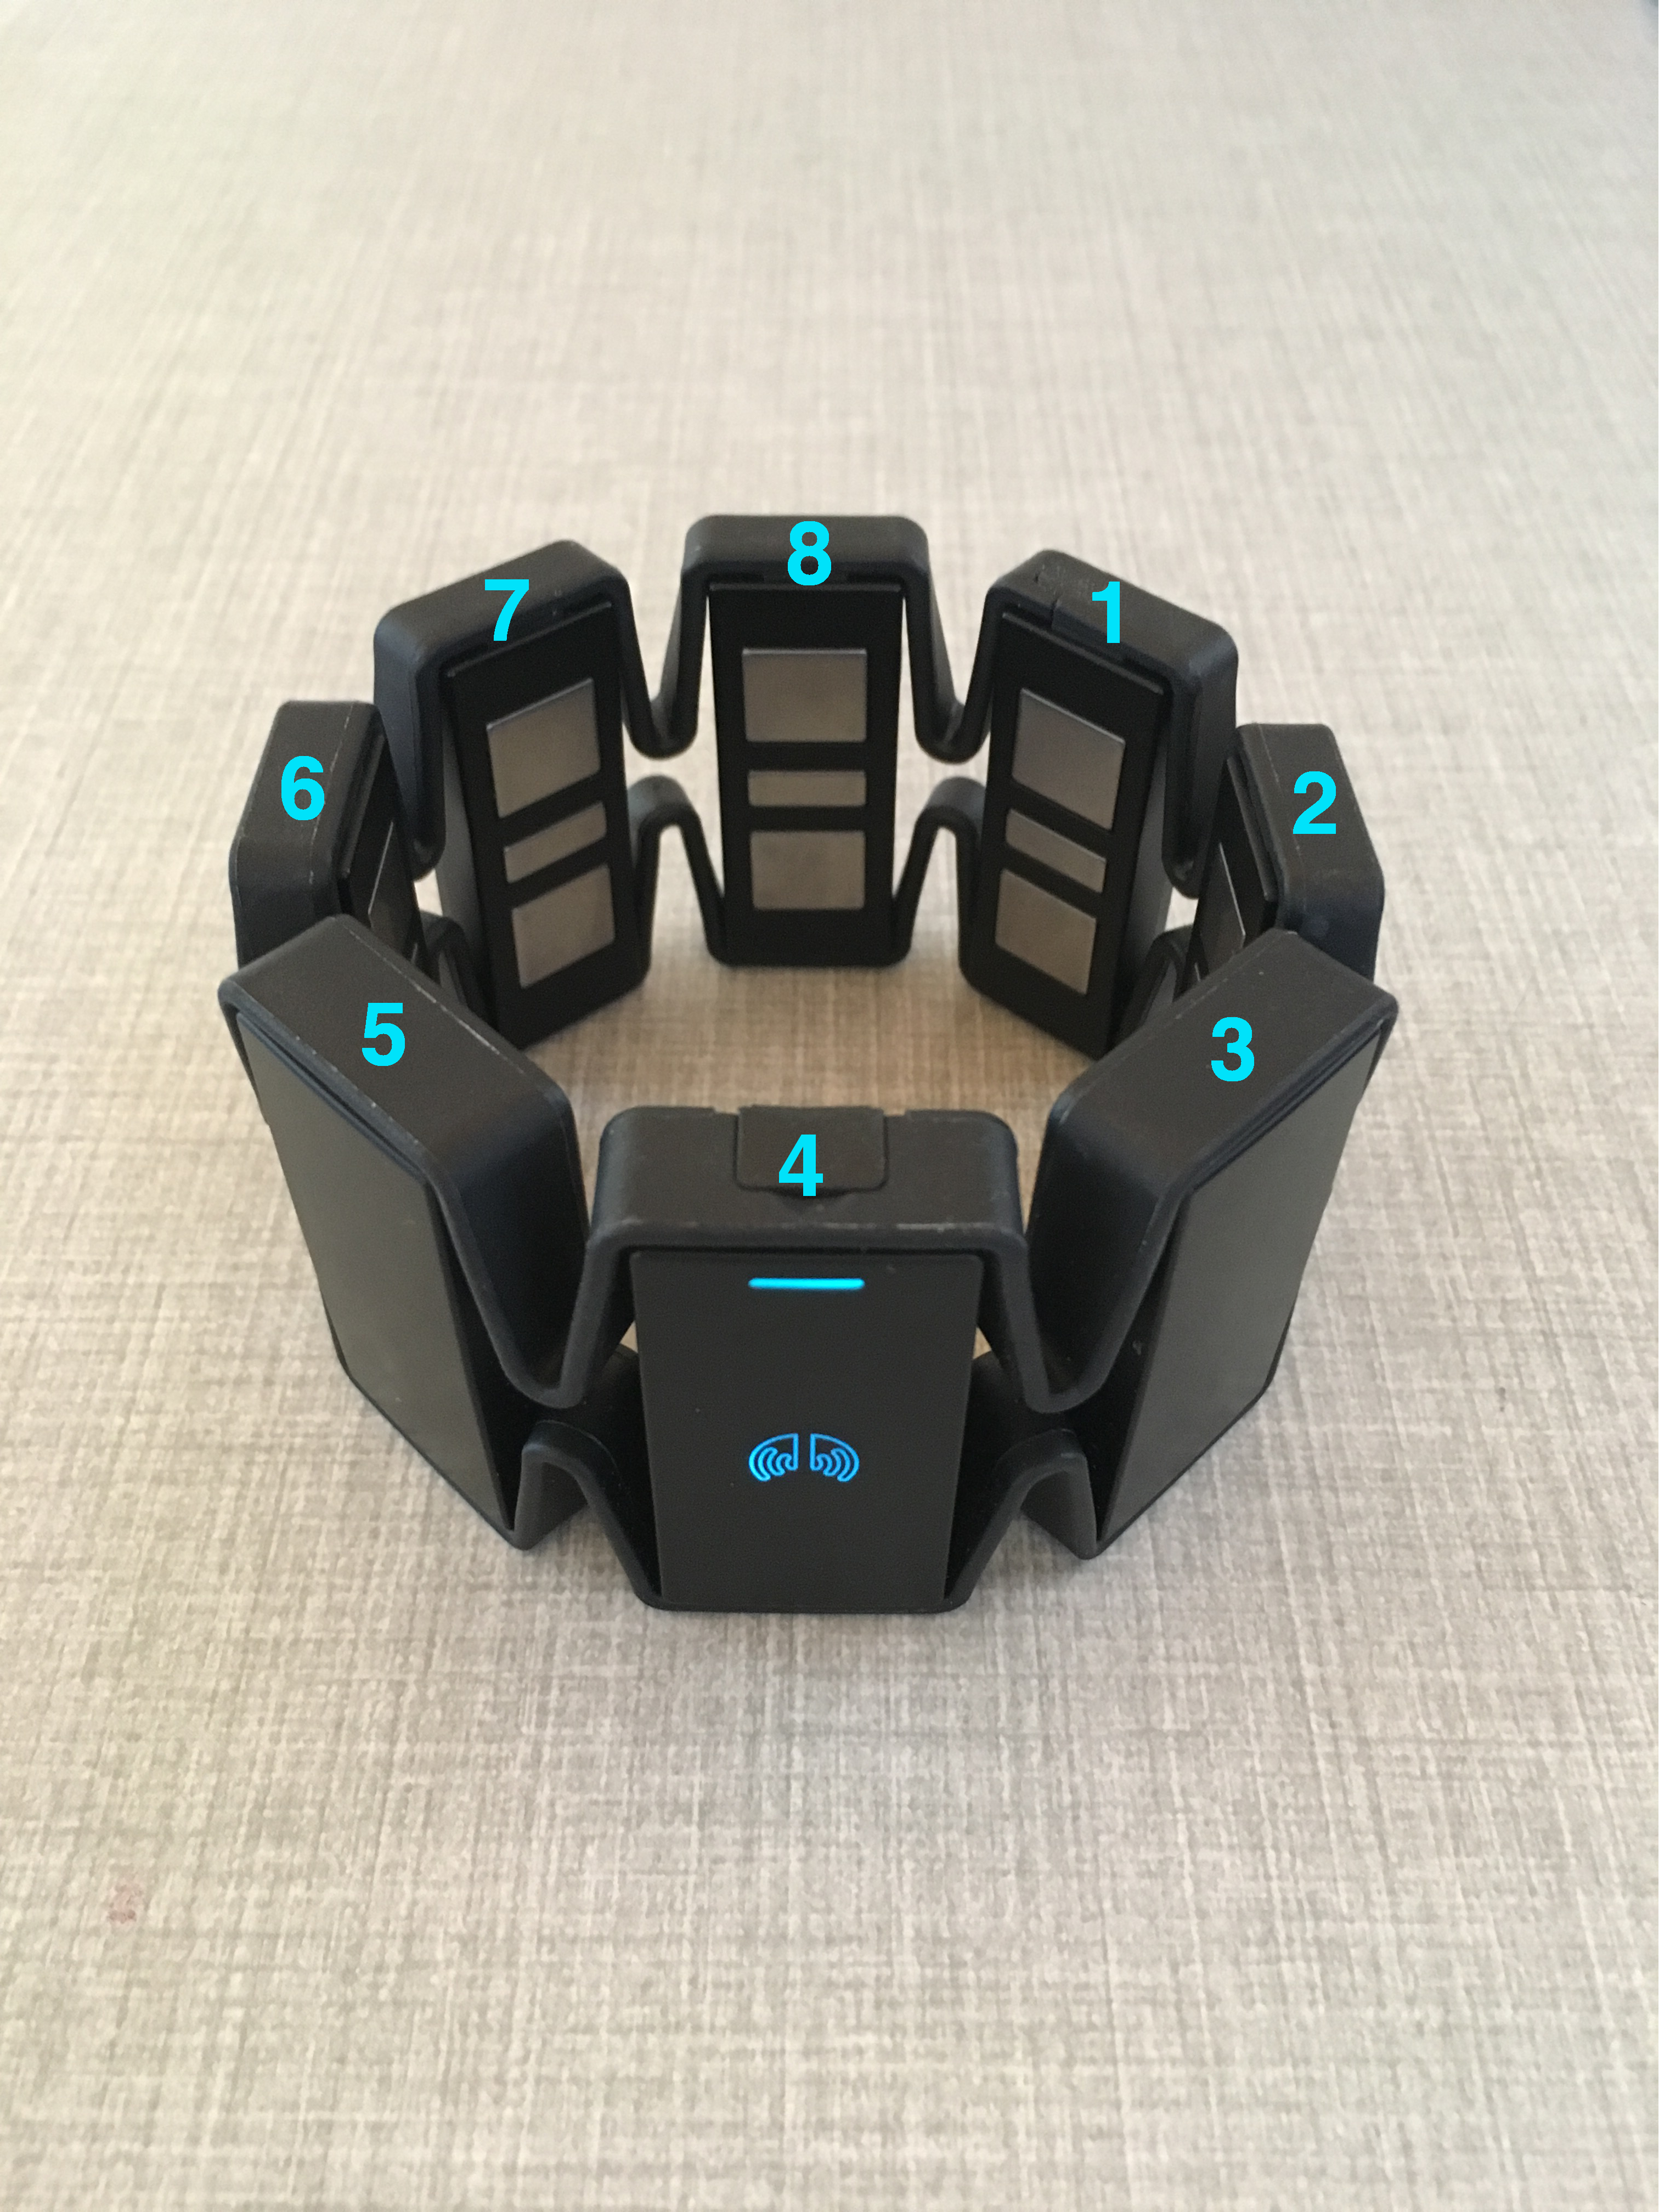
\includegraphics[width=.4\textwidth]{figures/xBackground/myoband}  
	\caption{MYB from Thalmic Labs. The number on each channel indicates which channel corresponds to which column in the digital output, when acquiring data from MYB.}
	\label{fig:myoarmband} 
\end{figure}

When initiating the wearing of the armband there is two calibration phases the user must follow before the armband is ready to use - the warm-up phase and the sync phase. During the warm-up phase the armband is ensuring a strong electrical connection with the muscles in the forearm as possible. This is mainly provided by light sweating on the skin under the electrodes, which improve the connection similar to electrode gel \cite{Cram2012}. During the sync phase, the armband determines its orientation in space, position on and which arm it is placed on. The MYB works better when fitted tightly on the thickest part of the forearm. For users with smaller forearms a set of clips can be added for the armband to get a constrained grip. \cite{Myoarmband2013}

\section{Data Processing} \label{sec:BG:dataProcessing}


In order to use the acquired EMG signal in myoelectric prosthetic control, it first has to be processed. %, which is referred to as pre-processing, as it is a processing procedure that is done before further processing is performed. 
Since the acquisition and most processing is done in the MYB before Bluetooth transmission, further processing of the signal is moderate. In myoelectric prosthetic control, several features are extracted from each electrode-channel for use in control, instead of using the raw EMG signal. Thus, the amount of information given to the control system is increased compared to only providing the raw EMG signal to the control system. The following two sections will briefly describe theory behind filtering and feature extraction in relation to this project. 
%As described in \secref{sub:BG:MYB} the MYB has some build-in degree of signal filtering. Data received from the MYB is therefore not \textit{raw} as in a completely untouched EMG signal. However, the signals received from the MYB will from this point on be described as the raw EMG signal, since the EMG signal has not been processed by any of the implemented filtering specific for this study.


\subsection{Filtering} \label{sub:BG:filtering} %\label{sub:filt}

Filtering is a cornerstone in preparing an EMG signal for any kind of use. The frequency spectrum of EMG is 10 Hz to 500 Hz. \cite{Cram2012} According to the Nyquist theorem, to achieve a loss-less representation of the signal the sampling frequency must be at least twice the maximum frequency of interest of the original signal \cite{Pozzo2004}. Additionally, EMG is sensitive to movement artefacts and electrical interference. Due to these circumstances, filters are often implemented to remove these unwanted contributors \cite{DeLuca2010}. 
General practice in filtering the EMG signal will include implementing a notch filter with very narrow width and steep slope, at frequencies 49-51 Hz or 59-61 Hz depending on the power supply. The intent is to remove any electrical interference noise. In the low frequency spectrum several recommendations (5 Hz, 10 Hz and 20 Hz) has been made for optimal corner frequency of a high-pass filter to remove movement artefacts. A low pass filter is also typically used to remove any noise and unwanted signal above 500 Hz \cite{Cram2012}. 

This project will utilize a MYB for data acquisition and as mentioned in \subref{sub:BG:MYB} the MYB has a sample rate of 200 Hz. In relation to this project a sampling frequency of at least twice the maximum of the recorded signal is not possible \cite{Cram2012}. This would require a sample rate of at least 1000 Hz, which cannot be achieved due to limitations in the MYB. Under other circumstances it would be astute to implement an anti-aliasing filter. However, this is not possible with the MYB since an anti-aliasing filter should be implemented before the sampling, when sampling below twice the bandwidth of the signal. %As this happens inside the MYB as fabricated by Thalmic Labs it is impossible to change for this project. 

%The effect of the low sample rate of the MYB is aliasing in the recording, causing a frequency component not originally in the EMG signal. To account for this it would be resourceful to implement a low pass filter to act as an anti-aliasing filter.  

\subsection{Feature Extraction} \label{sub:BG:featureExtraction} % \label{sub:BG:featureExtraction} %\label{sub:fe}
The input signals used for myoelectric prosthetic control are features based on the raw EMG signal. This increases the amount of information given to the control system, which facilitates more robust pattern recognition. \\
There are numerous feature components from an EMG signal which can be extracted either from the time-domain, frequency-domain, or time-frequency domain. Most used are features from the time- and frequency-domain. Time-domain features can be categorized in five different types based on their mathematical properties: energy information, complexity information, frequency information, prediction modelling and time-dependency. Extracting features from the frequency-domain requires a frequency transformation, calculating the spectral properties of the recorded signal, which takes up longer processing time than simply using time-domain features. 
Time-domain features are often chosen based on their quick and easy implementation as they do not require any transformation before extraction and are calculated based on the raw EMG signal. In addition, it is important not to choose redundant features for the classifier. \cite{Phiny2012}% which would be to chose features providing similar information. \cite{Phiny2012} \\
Extracting features for real-time prosthetic control is done by taking segments of the continuous signal, called windows. Calculation on extracting features are done in these discreet windows. This is done instead of using the instantaneous value due to the signals random nature. These windows are often overlapped to create a dense information stream for extraction. The relationship between window and overlap length is significant, when trying to determine the best representation. The window length is a matter of getting enough samples to do the calculation, but too long a window will result in delays slowing the control. Smith et al. \cite{Smith2014} found that the optimal window length in a classification control scheme that enables best performance ranges from 150-250 ms. Overlapping the window is a method to faster acquire windows by reusing a determined last segment of the prior window. The amount of overlap is a compromise between classification quality and responsiveness of the prosthesis; a large overlap will provide a shorter output delay, but a worse classification and vice versa \cite{Farrell2007}.

\section{Linear Discriminant Analysis}

Linear discriminant analysis(LDA) is a supervised classification method used to separate classes of data by linear decision boundaries. Each decision boundary is a hyperplane $H$ from which the minimum distance from the classes it separates is maximized, and the distance from the means of the classes are maximized. A decision boundary is defined as a linear combination of the feature values x and is given as:

\begin{equation}
g(x) = w^tx +w_0
\end{equation}

where $w$ is a weight vector deciding the orientation of $H$, and $w_0$ is a bias deciding the position of the hyperplane in relation to the origin. In a two category case the decision rule for deciding class $w_1$ or $w_2$ is: decide $w_1$ if $g(x) > 0$ and $w_2$ if $g(x) < 0$. $g(x) = 0$ then defines the decision boundary that separates the features into two decision regions $R_1$ for $w_1$ $R_2$ for $w_2$. $w$ is normal (orthogonal) to any vector on $H$, which can be used to calculate the distance $r$ from feature values to the decision boundary:

\begin{equation}
r = \frac{g(x)}{||w||}
\end{equation} 

From origin the distance is given as $\frac{w_0}{||w||}$, where if $w_0 > 0$ the origin is on the positive side of the decision surface, and if $w_0 < 0$ the origin is on the negative side. In the case of $w_0 = 0$ the decision surface passes through origin. In \figref{geolda} a geometric illustration of the linear discriminant function and its properties  is depicted.

\begin{figure}[H]                 
	\includegraphics[width=.4\textwidth]{figures/xBackground/geolda}  
	\caption{A geometric illustration of the linear decision surface $g(x)$ that separates the feature space into two decision regions $R_1$ and $R_2$. \cite{Duda2000}}
	\label{fig:geolda} 
\end{figure}

In a multicategory case $c$ decision boundaries are defined. The approach for defining the decision boundaries is given as:

\begin{equation}
	g_{i}(x) = w^tx_i +w_{i0} ~~~~~~~~~~~ i = 1,...,c,
\end{equation}

where $x$ is assigned to $w_i$ if $g_i(x) > g_i(x)$ for all $j \neq i$. This type of classifier is called a linear machine, and will be adopted as classification method in this project. 


\subsection{Generalized discriminant function}


\subsection{Gradient descend/minimum criterion function}


\subsection{Classification scores}
Evaluating the certainty that a feature value belongs to a given class can be done by computing the posterior probability of each class. The posterior probability is a value between 0 and 1, and is calculated as follows:

\begin{equation}
P(w_j|x) = \frac{P(x|w_j)P(w)}{P(x)}
\end{equation}

, where $w_j$ represents a class and x represents a feature value. The posterior probability is given as the product of the class conditional probability, $P(x|w_j)$ and the prior $P(w)$ divided by a normalization term $P(x)$ that guaranties that the posterior probabilities for all classes sums to one. $P(x|w_j)$ is the probability of obtaining a feature value when selecting samples randomly from a class. $P(w)$ is the likelihood that a sample from a class appears compared to the other class before it actually has appeared. 

%background regression 
\section{Linear regression methods} \label{sec:BG:linearRegressionMethods}
Classification can be used together with regression methods to provide a combination of the two in a control scheme. The output from the LDA classifier can be set to only decide on which movement is performed, and not
%The output from the LDA classifier only decides on which movement that is performed, and not 
at which contraction level the muscles used in the given movement are performing. Thus, the prosthesis can not perform any movement if only using the classification output.  In statistics linear regression is often used to determine relations between variables. This notion can also be applied for myoelectric prosthetic control. While classification only provides an output on which class is recognized, a linear regression model provides a continuous output value based on the input value. If the regression model is fitted with information on different contraction levels for a given movement, control proportional to the contraction level will be achieved \cite{Hwang2017, Hahne2014, Bruun2017}. In the overall control scheme the classifier can then be used to decide which movement is performed, and a regression model can decide at which contraction level the movement is performed at. Similarly as with the classifier, regressors needs to be trained based on data acquired from the user, where the features extracted from the raw EMG signal is used as input. This procedure is described in the following section. 
%The use of linear regression is often used in statistics to determine relations between variables. Regressions methods also has its use in control schemes of myoelectric prosthetics \cite{Hwang2017, Bruun2017, Hahne2014}. The difference between classification and regression is that classification attempt to classify similar patterns in recordings, between previously acquired data and new data, while regression methods provide a continuous output value based on the input value \cite{Mendez2017, Hahne2014}. %\fxnote{sidste sætning er taget fra indtroduktionen men det stykke skal nok skrives om/væk alligevel for det omhandler classifikation VS regression. edit: er taget ud af introduktionen nu.}

Different models of linear regression exist to account for different uses. When utilizing regression methods it must be considered what the input and output variables are what type of relation these variables might have. The appropriate regression model must then be applied. Simple linear regression approximate a relation between one dependent variable $Y$ and one independent variable $X$ \cite{Zar2009}:

\begin{equation} \label{eq:simpleLinearRegression}
Y = \alpha + \beta X + \epsilon
\end{equation}

where $Y$ is the control output for the prosthesis, $X$ is the feature extracted from the EMG signal, $\beta$ is the regression coefficient in the sampled population, $\epsilon$ is the error, and $\alpha$ is the predicted value of $Y$ at $X = 0$.
This model can be expanded to estimate relations between one dependent variable and several independent variables. This is called multivariate regression and expands on the equation of simple linear regression, given in \eqref{eq:simpleLinearRegression} \cite{Zar2009}:

\begin{equation} \label{eq:multiLinearRegression}
\hat{Y} = \alpha + \beta_1 X_{1} + \beta_2 X_{2} + ... + \beta_i X_{i} + \epsilon_i
\end{equation} 

where $i$ in this project would correspond to the number of channels in the MYB \cite{Zar2009}. Since this regression model approximates the relation between several independent variables and one dependent variable, this model can be used as a control scheme in myoelectric prosthetics. Here the channel-recordings of muscle activity can be considered independent variables, and used to estimate one control output, which would be the dependent variable. \cite{Bruun2017}



\section{User training} \label{sec:BG:userTraining}

As user training in relation to prosthetic control is the main focus of this project an understanding of this concept in relation to receiving a prosthetic device is of great importance. Therefore the following section will cover an introduction to the concept of user training and its importance when preparing a subject to receive a prosthetic device. In addition some of the prior techniques of conducting user training will be presented, facilitating the possibility of assembling a user training protocol based on the most recent and cutting edge results. \\
%user training and implementation
When fitting an amputee with a prosthesis, the way the prosthesis is controlled is important. A lot of work lies both ahead and behind fitting a person with a prosthesis. When developing and manufacturing a prosthesis two concepts emerge, one being system training and the other being user training. System training is training the control system to be able to recognize and differ movements based on the EMG-signal being fed to the system. \cite{Fougner2012} User training on the other hand focuses on training the user in performing distinguishable movements which can be recognized by the control system. Here different types of feedback can be used to inform the user on how well the user performs a movement or how well the system recognizes the users performed movements. \cite{Powell2014,Simon2013} \\
%Copied from introduction 
Only few studies have earlier explored the optimal way of giving visual feedback in user training \cite{Jiang2012}. In a 2014 study Powell et al. \cite{Powell2014} provided the user with real-time visual feedback of a virtual prosthetic. This type of feedback is similar to the visual feedback a prosthesis user would receive using a normal prosthesis, although without the sensory feedback of the weight of the prosthesis. Pan et al. \cite{Pan2017} provided a visual feedback of an arrow to be moved on a 2D plane. The arrow was controlled by two DOF's; one controlled the horizontal position of the arrow, while the other could rotate the arrow \cite{Pan2017}. Fang et al. \cite{Fang2017} provided real-time visual feedback of subjects performed movement in relation to the classes defined in the system. The feedback visualized a map of clusters of different classes which subjects could match the position of a cursor to. When subjects could match the cursor to the centroid of a cluster the performed movement corresponded the best with the class of that movement. \cite{Fang2017} All studies observed an improvement in user performance after being exposed to focused user training with visual feedback. 

A 2013 study by Scheme et al. \cite{Scheme2013} proposed a novel approach of utilizing confidence-based rejection to improve system training of myoelectric control. Here a classification control scheme was provided with confidence scores to assist in acceptance or rejection of the class output. The confidence scores were calculated from a modification of Bayes' theorem. Scheme et al. \cite{Scheme2013} showed a significant improvement in performance with the use of the rejection-capable system when compared to the normal classification scheme. A similar approach could be used in user training by providing the confidence scores of the classification to the user as a form of visual feedback. \\
Thus, this study propose a novel method of providing users with feedback containing confidence scores for different classes in a classification control scheme during user training. Contrary to current feedback methods in user training this approach could enable users to better understand how the classification works based on their performed movements. During user training this could improve the way users perform specific movements in order to enable the system to better recognize and classify movements correctly.


\section{Validating Performance} \label{sec:BG:validatingPerformance}

Measuring the performance of achieved prosthetic control cannot be seen as a trivial task, and different approaches can be used. The achieved performance can be measured by affixing a prosthesis on to the test subject and validate performance hereby. Often, like the current project, the subjects do not consist of actual amputees but instead healthy subject. In these cases, the performance validation is done by implementing a virtual test environment where the subjects is to control an object on the computer screen by performing movements. The following section will further elucidate the procedures of such a virtual test for validating prosthetic control.      


\subsection{Modified Fitts' Law} \label{sub:BG:fitts}

Fitts' Law test is a common method of quantifying performance of movements, first proposed by Paul M. Fitts in 1954 \cite{Fitts1954}. Fitts' Law states the that time required to reach a targeted area is a function of the width and distance of the target. The output of a Fitts' Law test is the throughput, as given by \eqref{eq:TP}. This measure gives an idea of the trade-off between speed and accuracy. A modified Fitts' Law test designed for a virtual 2D and 3D target acquisition test has later been used by \cite{Kamavuako2014} and \cite{Scheme2013} respectively. Here, four additional metrics were added in an real-time test, where a virtual computer cursor was used to represent the control output \cite{Scheme2013, Kamavuako2014}. The four additional metrics, path efficiency, overshoot, stopping distance and completion rate, were made by \cite{Poulton2013} and \cite{Simon2011}. While the throughput measure from the conventional Fitts' Law test is usable, it does not cover all aspects of the control required to complete a test. The additional four measures were added to quantitatively assess performance of naturalness, spontaneity, and compensatory motions during use. The total five proposed performance measures in assessing myoelectric control are \cite{Scheme2013a}: 

Throughput (TP) which represents the trade-off between speed and accuracy. TP uses the relationship of time taken to reach a certain target in seconds ($MT$) and the index of difficulty (ID). This forms: \cite{Scheme2013,Fitts1954}

\begin{equation} \label{eq:TP}
TP=\frac{1}{N}\sum_{i=1}^{N} \frac{ID_i}{MT_i} 
\end{equation}

where $i$ is a specific movement and $N$ is the total number of movements. ID relates to the target distance $D$ and width $W$. The ID for each target, from the origin to a specific target of a certain size is calculated using \cite{Scheme2013,Fitts1954}:

\begin{equation} \label{eq:ID}
ID=log_2(\frac{D}{W}+1)
\end{equation}

Path Efficiency (PE) describes the quality of control by making a measure of the straightness of the cursor's path to the target, by making a ratio of the actual path distance versus the optimal path distance. This tests the users' ability to continuously control the cursor position. Following the optimal path will result in a PE of 100\%. PE is calculated as follows \cite{Scheme2013, Poulton2013}:       

\begin{equation} \label{eq:PE}
PE = \frac{Optimal ~ Distance}{Actual ~ Distance}
\end{equation}		 

Overshoot (OS) is the number of times the cursor enters and then leaves the target before the dwell time inside the target is reached, across all target in the test, divided by the total number of targets. OS tests the users ability to control the velocity of the cursor accurately. A perfect OS-score of zero is reached if the cursor dwells within the target boundaries on the first try for all targets, and is calculated as the following \cite{Scheme2013, Poulton2013}:

\begin{equation} \label{eq:OS}
OS = \frac{Total ~ Number ~ of ~ Overshoots}{Total ~ Number ~ of ~ Targets}
\end{equation}

Stopping Distance (SD) describes the users ability to rest and thereby perform no movement. The SD measure is the distance moved during the dwell time across all targets, and is given as \cite{Scheme2013}:

\begin{equation} \label{eq:SD}
SD = \sum_{i=1}^{N} (Distance ~ Inside ~ Target)_i
\end{equation}

where $i$ is a reached target and $N$ is the total number of reached targets.

Completion Rate (CR) describes the percentage of targets reached within the total allowed time. This gives a general idea of the user's performance, and is calculated as \cite{Scheme2013,Simon2011}: 

\begin{equation} \label{eq:CR}
CR = \frac{Number ~ of ~ Reached ~ Targets}{Total ~ Number ~ of ~ Targets}
\end{equation}

\section{Data separability} \label{sec:BG:dataSeparability}
Besides evaluating the user performance in real-time, it would be beneficial to evaluate the clustering of feature values used to fit the classifier and regressors off-line. This will provide information on how the clusters between classes separates and how the feature values within clusters bundle. %Thus it can be evaluated between sessions if the clusters are more distinguished and thereby easier for the classifier and regressors to discriminate between. 
By doing this between sessions it can be evaluated how distinguishable the clusters are to judge how well the classifier and regressors will discriminate between the different clusters. For this purpose a Principle Component Analysis (PCA) will be utilized to reduce the dimensionality of the feature space, from which is subsequently can be used to calculate the distance between clusters and distances from feature values to centroids within clusters. The following section provides theoretical information on the PCA procedure. 


\subsection{Principal Component Analysis} \label{sub:BG:PCA}
PCA is used to express a set of possibly correlated variables into uncorrelated components, called principal components (PC). A dataset of many variables can thus be expressed in a reduced dimensionality hyperspace using less variables that are the most defining for the given dataset. Each principal component is orthogonal on the former and are uncorrelated and have zero covariance. They each define the largest variance in an axis, such that the first PC describes the direction of the maximum variance of the dataset. Each following PC describes the next highest variance of the dataset, with the constraint that it is orthogonal and has zero covariance with any of the former PCs. \cite{Semmlow2014}
PCA is the orthogonal projection of data onto a lower dimension linear space. A PC is found by minimizing the variance by projecting the feature values, the red dots in \figref{projection}, onto the line describing the highest variance in the data set (purple line) as seen on \figref{projection}. The PC (purple line) is found by minimizing the mean square distance between the data points. \cite{Semmlow2014}

\begin{figure}[H] 
	\includegraphics[width=0.3\textwidth]{figures/zASP/projection}
	\caption{Projection of feature values (red dots) onto PC axes (purple).}
	\label{projection}
\end{figure}
\vspace{-10pt}
The algebraic method of calculating the PCs can be done by using Singular Value Decomposition (SVD). The first step is to compute the squared cross product matrix of variances and covariances among every pair of the variables in the data set, where the diagonals are the variances and the off-diagonals are the covariances, as done in the following equation \cite{Semmlow2014}:
%\vspace{-20pt}
\begin{equation}
S = X \textquoteright X
\end{equation}
Where S is the cross product and X is the feature set matrix. When finding the PCs it includes an eigen-analysis of S. The eigenvalues of are solutions to the following equation \cite{Semmlow2014}:
%\verticalspace{1}
\begin{equation}
| S - \lambda I |  = 0
\end{equation}
Where $\lambda$ is the variance of each PC and $I$ is the identity matrix. After solving for $\lambda$ the eigenvectors can be solved through the following equation \cite{Semmlow2014}:
\begin{equation}
det | S - \lambda I | b_{i} = 0
\end{equation}
Where $b_{i}$ is used to calculate the eigenvectors as in \cite{Semmlow2014}:
\begin{eqnarray}
u_{i} = \frac{b_{i}}{\sqrt{b_{i}^{\textquoteright} b_{i}}}
\end{eqnarray}
Where $u_{i}$ is the $i^{th}$ number of eigenvectors. The number eigenvectors equal the dimension size of the original feature space. 
The SVD orders the eigenvalues by size, so that $\lambda_{1} > \lambda_{2} … > \lambda_{i}$. The scores for each PC is equal to the corresponding eigenvalue for that exact axis. The eigenvalues describe how much of the variance is accounted for by the associated PC. Summation of all eigenvalues accounts for the total variance of the data set; this is called the trace. To find how much the each PC accounts for, the eigenvalue of that PC is divided by the total variance: $\%~ of~ total~ variance~ = \frac{\lambda_{i}}{Trace}$. Deciding how many PCs the feature space should be reduced to, by setting a threshold of how much of the total variance should be preserved. \cite{Semmlow2014}

\subsection{Distance measure} \label{sub:BG:distanceMeasure}
After reducing the dimensionality of the original feature set the clusters can be analysed. For the purpose of measuring distances between and within clusters the centroid of each cluster must be calculated, as in \eqref{eq:centroid}:

\begin{equation} \label{eq:centroid}
	C = \Bigg[ \frac{[x_1+x_2 +~...~+ x_i],[y_1+y_2 +~...~+ y_i] ,~...~,[k_1+k_2 +~...~k_i]}{k} \Bigg]
\end{equation}

Where $C$ is the centroid, $i$ is the number of feature point in a dimension and $k$ is the number of dimensions. To calculate the distance between centroids of clusters the Euclidean distance (ED) is computed. The ED is the length of the a line segment connecting points, in this case in form of two centroids $p$ and $q$. The calculation of ED in a $k$-dimensional space is as in \eqref{eq:euclidiandistance}:

\begin{equation} \label{eq:euclidiandistance}
	ED(p,q) = \sqrt{(p_1-q_1)^2 + (p_2-q_2)^2~+~...~+ (p_k-q_k)^2}
\end{equation} 

When calculating the distance from feature values in a cluster to their corresponding centroid the ED is computed likewise. To get a general impression of the distance from the feature values constituting the cluster to the centroid of the cluster the average of the distances is calculated. 

from feature values of a cluster to their centroid, the average distance from all feature values to their centroid is calculated. 





%\section{Statistical analysis}
When evaluating the scores obtained in the performance test a statistical analysis is used. For this project a Friedman's test will be utilized is due to a small sample population, and because it is assumed that the probability distribution of the performance scores is unknown. Friedman's test is commonly used to test if different treatments have similar or different effects in a subject population. In the case of this project it is used to test whether performance in prosthesis control is similar or different across sessions in a subject population and if performance scores differ or bear resemblance between two subject populations. In the following section, theory on how the Friedman's test is calculated will be presented.

\subsection{Friedman's test}
When testing a subject population of a given number of measurements the measurements must first be arranged in columns, where each column corresponds to a certain measurement, and each row corresponds to one subject. Each row must then be ranked separately, where the smallest number is ranked 1. If numbers in a row are equal they get the mean of the rank they would have received. The sum $R$ of each column is calculated, and the number of measurements $k$, number of subjects $n$ is used to calculate the Friedman's F value in the following equation:

\begin{equation}
	F = \frac{12}{n \cdot k \cdot (k+1)} sum_{i=1}^{k} R_{i}^{2} - 3 \cdot n(k + 1)
\end{equation}

The critical value of F is then determined by looking in a table of critical values for Friedman's test. 

The p-value indicates whether the null-hypothesis is to be rejected and an alternative hypothesis should be accepted; where the null-hypothesis expresses no relationship between measurements and the alternative hypothesis expresses a relationship between measurements. A p-value of 0.05 is usually used to as significance level. If the p-value is under 0.05 the null-hypothesis is rejected and vice versa. 





 
%nævn om hvad h0-hypoteserne præcist er i metode afsnittet

%"The term "null hypothesis" is a general statement or default position that there is no relationship between two measured phenomena, or no association among groups. Rejecting or disproving the null hypothesis—and thus concluding that there are grounds for believing that there is a relationship between two phenomena (e.g. that a potential treatment has a measurable effect)"


\chapter{Methods} \label{chap:Methods}
The background chapter covered the basic procedures associated with myoelectric prosthetic control and techniques to deal with the proposal of improving users' ability to operate a myoelectric transradial prosthesis by training the user with visual confidence score feedback. This involves descriptions of different hand movements, how the EMG signal is generated and acquired with surface EMG electrodes using the MYB and how the raw EMG signal is processed before it is segmented in windows. Furthermore, it was described how features are extracted from the segmented signal, how the feature values are used in a classification control scheme to distinguish which movement is performed, how linear regression models are used to obtain proportional control, how confidence scores can be calculated as posterior probabilities from the classification scheme, how user training previously has been used to optimize users' ability to operate a myoelectric transradial prosthesis and how the user performance is evaluated. \\
The information acquired in the background section will lay foundation for how the study will be designed, how the procedures will be implemented and which considerations that have been made regarding the implementation. This will be covered in the methods chapter. As the project investigates whether users' ability to operate a myoelectric prosthesis can improve after training with confidence score as visual feedback, a major focus has been put in the implementation of the user training. The chronology of the methods chapter is that the study design will be presented first, after which the implementation of the different procedures will be presented, as the procedures are implemented with regards to how the study design is formed. 

\section{Study Design} \label{sec:M:studyDesign}

This experiment focused on training the user to improve prosthetic control on a classification-based control system. The novel approach in this study was to provide the user with visual feedback on how the system recognized the performed movements during user training, by showing the confidence scores of the movements the control system recognized. The following section will lay an overview of the structure of this experiment. \\
To test if myoelectric prosthetic control could be improved by using visual confidence score feedback the following research hypothesis was made: 
\begin{center}
	\textit{Exposing subjects to user training, in which confidence scores of movement recognition is used as visual feedback, will show statistically significant improvement in performance in a Fitts' Law test compared to a control group receiving label feedback.}
\end{center}


To test the hypothesis 16 subjects of mean age 25.3 $\pm$ 1.48 were recruited: 15 male and 1 female where 14 were right handed and 2 were left handed. Subjects were randomly assigned to either a control group or test group with 8 subjects in each group. The subjects enrolled were assessed to meet inclusion criteria presented in the experimental protocol for test subjects. The experimental protocol was handed out to the test participants before starting the experiment. Subjects in the test group received the experimental protocol containing specific guidance on how to perform the intended user training. The control group as well received the experimental protocol giving guidance on how to perform the user training intended for the control group. The experimental protocol containing both user training guidance schemes can be found in \secref{sec:protocol:experiment}. During the experiment the subject was seated on a chair, with the dominant arm wearing the MYB hanging relaxed laterally down the torso as seen on \figref{fig:experiment_setup} in the experimental protocol. \\
The experiment was designed as a three session investigation. In each session both groups had data acquired, received user training and did a performance test through a Graphical User Interface (GUI) developed in MATLAB (2017b). During session one it was chosen to add a performance test before exposing the subjects to user training. This preliminary performance test was set to act as a baseline for each group to highlight any initiating group disparity. A graphical illustration of the stages of the study design can be seen on \figref{fig:std}. Essential for the experiment was the difference in user training highlighted in step 3, where the groups received two different types of visual feedback. The test group received a visual feedback of the confidence score the classifier produces, when the subject train the different types of movements. The control group received the same visual training, however this would not inform of the confidence score but instead solely show which movement the classifier thought was being performed. The sections to come will further elaborate on the implementation of each element in the experiment and how the user training differs.  

\begin{figure}[H]                                         
	\includegraphics[width=0.64\textwidth]{figures/pMethods/OLDStudy_design}  
	\caption{Graphical illustration of the experiment showing the steps of each session for the test and control group. Highlighted is user training in step 3 which is the only procedure that varies between the two groups, and thus the area of research interest in the experiment.}
	\label{fig:std} 
\end{figure}   

%data acquisition
\section{Data Acquisition} \label{sec:M:dataAcquisition}

This section will clarify the method of acquiring data in this project. For data acquisition the MYB was used to record EMG signals from muscles in the forearm. The recordings were made on test subjects instructed to perform six different hand gestures as introduced in \secref{sec:BG:anatomy}. 


%As described in \secref{sec:MYB} about the MYB, the armband has a sample rate of 200 Hz. 
%According to the Nyquist theorem, to achieve a loss-less representation of the signal the sampling frequency must be at least twice the maximum frequency of interest of the original signal \cite{Pozzo2004}. In relation to this paper a sampling frequency of at least twice the maximum of the recorded signal is not possible, since muscles of the forearm have a maximum frequency of 400-500 Hz \cite{Cram2012}. This would require a sample rate of at least 1000 Hz, which cannot be achieved due to limitations in the MYB. The effect of the low sample rate of the MYB is aliasing in the recording, causing a frequency component not originally in the EMG signal. To account for this an \textbf{anti-aliasing filter is implemented}, described further in \secref{sec:prePros} on preprocessing of the signal. Thus, data will be acquired as a sampling frequency of 200 Hz.

For acquiring data a Graphical User Interface (GUI) was designed. In the GUI the possibility to change settings for different types of recordings was implemented. The first type of recording was a baseline measurement. This recording was made in order to be able to reduce the baseline noise. This was done by subtracting the baseline from the EMG signal when the the EMG signal reached higher than the baseline. When the EMG signal was below the baseline, it was set as 0. \\
The second recording type was a Maximum Voluntary Contraction (MVC) which was a 15 second recording of the subject's maximum contraction of one movement that could be kept constant for 15 seconds without developing muscle fatigue. The mean MVC across all channels was set as a reference value for the following recordings. \\
The third type of recording was of EMG signals used to train the control system. The recordings of EMG signals were based on fractions of the MVC, which could be set using a menu in the GUI. As stated in \secref{sec:M:usertraining}, three contraction levels was used: 40\%, 50\% and 70\%. The level of contraction defined the height of the plateau of a trapezoid trajectory which would be plotted in a window in the GUI. When doing EMG recordings the subjects must perform the instructed movement to control the height of a cursor in the trapezoid plot to best match the trajectory of the trapezoid. The cursor height was calculated as the mean EMG signal across channels normalized based on the MVC. The subject only controlled the height (EMG intensity) of the cursor as the cursor would automatically move forward along the x-axis in relation with time. The recording time was 15 seconds: 2.5 seconds rest at the initiation and ending, 2.5 seconds on the trajectory incline and decline and 5 seconds on the plateau. Of the recorded time only the plateau phase and the last second of the incline and first second of the decline were used to fit the classifier. This approach provided data from a performed movement in both the transition and steady state phase. This data acquisition method was applied since the use of dynamically changing force data in training a classification-based control scheme has shown to improve performance and tolerance to proportional control \cite{Scheme2015}. 
During recordings the investigators evaluated whether the subject followed the trajectory well enough. Furthermore to evaluate the training data, the investigators observed a spider-plot during the acquisition, which was seen on the right side in the GUI. The spider-plot showed the amplitude output for each channel in the MYB. If the activation pattern of the channels changed dramatically, it was a sign of fluctuations in muscle activation, and thus the subject did not perform the instructed movement. If this was observed the recording was discarded and a new was be acquired. An illustration of the data acquisition GUI is shown in \figref{fig:GUIplot}.

\begin{figure}[H] 
	\includegraphics[width=1\textwidth]{figures/xBackground/dataacqGUI}
	\caption{The implemented data acquisition interface. On the left is different buttons shown, where only "Measure Baseline", "Measure MVC" and "Record Training Data" is used in the data acquisition. The "Contraction Level" menu forms the trapezoidal trajectory and "Movement Type" saves the performed movement the correct label. In the center is the trapezoidal trajectory and the cursor representing the EMG signal. On the right is the spider-plot used to evaluate the quality of the performed movement.}
	\label{fig:GUIplot}
\end{figure}



\section{Data processing}




\subsection{Filtering of signal} \label{sec:prePros} 

As earlier mentioned to counter the limitation in sample frequency imposed by the MYB an anti-aliasing filter has been implemented before further processing of the signal.  


The data obtained with MYB is acquired with a sample frequency of 200 Hz this propose the error of aliasing due to the non sufficient sampling frequency of at least twice the highest frequency \cite{Pozzo2004}. Furthermore it is recommended in \cite{DeLuca2010} to filter the low-frequency spectrum to counter artifacts of movement.



 Presented obstacles in both the low-frequency and high-frequency level of the acquired signal has lead to an implementation of a second-order bandpass filter from 10 Hz to 90 Hz. 

The figure shows aliasing in above 100 HZ 
result in the filter 

Also seen in the figure is the effect of the notch filter mentioned in \secref{sec:MYB}. The filtered signal clearly shows a drop in power around 50 Hz. 

put figure here 



\subsection{Feature extraction}

































\section{Building the Control System}

Following the data acquisition and processing, the training data obtained was used for movement classification. The features extracted for each of the seven movements were used for building the classification. The first subsection will cover the implementation of the classification and its output. An explanation of how the classification output for user training and control is used can be found in \secref{sec:M:usertraining} and \secref{sec:M:fittsLaw}. Furthermore to be able to read out the intensity of movements a regression based calculation is made. The implementation of movement intensity control will be explained in the adjacent section.   


\subsection{Movement Classification}

For classifying movements in this project the use of Linear Discriminant Analysis will be used as presented in \secref{sec:BG:classification}. The classifier is fed with the prior acquired training data in order to train the control system.  
The acquired training data were assembled in to matrices for each of the seven movements with one of the five features, containing the feature values for each of the eight channels. An example of one of these matrices can be seen in \eqref{eq:CCMatrix}. This matrix contains the feature values n, for the feature CC for all three intensities of extension across all eight channels.  

\begin{equation} \label{eq:CCMatrix}
AllIntCC\_Ex=\begin{bmatrix} 
\begin{bmatrix}
\ CCExtension40_{1,1}, CCExtension40_{1,2} \cdots CCExtension40_{1,8} \\ 
\ \vdots \qquad \qquad \qquad \ddots \qquad \qquad \qquad \vdots \\
\ CCExtension40_{n,1}, CCExtension40_{n,2}  \cdots CCExtension40_{n,8} \\ \end{bmatrix} \\
\begin{bmatrix} 
\ CCExtension50_{1,1}, CCExtension50_{1,2} \cdots CCExtension50_{1,8} \\
\ \vdots \qquad \qquad \qquad \ddots \qquad \qquad \qquad \vdots \\
\ CCExtension50_{n,1}, CCExtension50_{n,2} \cdots CCExtension50_{n,8} \\ \end{bmatrix} \\
\begin{bmatrix} 
\ CCExtension70_{1,1}, CCExtension70_{1,2} \cdots CCExtension70_{1,8} \\
\ \vdots \qquad \qquad \qquad \ddots \qquad \qquad \qquad \vdots \\
\ CCExtension70_{n,1}, CCExtension70_{n,2} \cdots CCExtension70_{n,8} \\ \end{bmatrix} \\
\end{bmatrix}
\end{equation}

As seen the matrix consists of three smaller matrices, one for each of the intensity as explained in \secref{sec:M:dataAcquisition}.  
The AllIntCC$\_$Ex matrix is just one of multiple as mentioned, to assemble a total training matrix to feed train the classifier all matrices are assembled into one big training matrix. This matrix can be seen below in \eqref{eq:AllMatrix}. 


\small \begin{equation} \label{eq:AllMatrix}
\begin{bmatrix} 
\ AllIntCC\_Ex, AllIntSMAV\_Ex, AllIntSMADR\_Ex, AllIntMADN\_Ex, AllIntWL\_Ex \\
\ AllIntCC\_Fl, AllIntSMAV\_Fl, AllIntSMADR\_Fl, AllIntMADN\_Fl, AllIntWL\_Fl \\
\ AllIntCC\_Rd, AllIntSMAV\_Rd, AllIntSMADR\_Rd, AllIntMADN\_Rd, AllIntWL\_Rd \\
\ AllIntCC\_Ud, AllIntSMAV\_Ud, AllIntSMADR\_Ud, AllIntMADN\_Ud, AllIntWL\_Ud \\
\ AllIntCC\_Ch, AllIntSMAV\_Ch, AllIntSMADR\_Ch, AllIntMADN\_Ch, AllIntWL\_Ch \\
\ AllIntCC\_Oh, AllIntSMAV\_Oh, AllIntSMADR\_Oh, AllIntMADN\_Oh, AllIntWL\_Oh \\
\ AllIntCC\_Re, AllIntSMAV\_Re, AllIntSMADR\_Re, AllIntMADN\_Re, AllIntWL\_Re \\
\end{bmatrix}
\end{equation}

\normalsize
The classifier is trained, by fitting the matrix presented in \eqref{eq:AllMatrix} with labels for each of the movements, making it a supervised learning method. The classifier thereby forms seven classes, one for each of the movement, with discriminative decision boundaries separating them. For calculating the real-time use of classification outcome and confidence scores in user training and performance test as intended, the predict function in MATLAB has been used. The function is continuously evaluating each sample to the different movement clusters in the five dimensional feature space, as theory explains in \secref{sec:BG:classification}. Hereby the sample is assigned to the cluster (movement) it is most likely to belong to based on the training data. The Predict function also calculates the probability membership for the sample to all classes giving an idea of how sure the classifier is and thereby indicating the correctness of the movement performed. 



\subsection{Proportional Control} \label{sub:M:regression}
To obtain proportional control linear regression models, regressors, for each movement were made. For this purpose multivariate linear regression was used, as explained in \secref{sec:BG:linearRegressionMethods}. To fit a regressor dependent and independent variables were needed. The independent variables were set as MAV features extracted from the raw EMG data from the data acquisition as explained in \secref{sec:M:dataAcquisition}. To ensure that the regressor did not produce an output during rest, the MAV features extracted from the raw EMG from a resting position were included as independent variables in each regressor. An example of the independent variables used to fit the regressor for the extension movement is seen in \eqref{eq:q:segMatrix}.

\begin{equation} \label{eq:segMatrix}
AllIntMAV\_Ex=\begin{bmatrix}
\begin{bmatrix}
\ MAVRest_{1,1}, MAVRest_{1,2} \cdots MAVRest_{1,8} \\ 
\ \vdots \qquad \qquad \qquad \ddots \qquad \qquad \qquad \vdots \\
\ MAVRest_{n,1}, MAVRest_{n,2}  \cdots MAVRest_{n,8} \\ \end{bmatrix} \\
\begin{bmatrix}
\ MAVExtension40_{1,1}, MAVExtension40_{1,2} \cdots MAVExtension40_{1,8} \\ 
\ \vdots \qquad \qquad \qquad \ddots \qquad \qquad \qquad \vdots \\
\ MAVExtension40_{n,1}, MAVExtension40_{n,2}  \cdots MAVExtension40_{n,8} \\ \end{bmatrix} \\
\begin{bmatrix} 
\ MAVExtension50_{1,1}, MAVExtension50_{1,2} \cdots MAVExtension50_{1,8} \\
\ \vdots \qquad \qquad \qquad \ddots \qquad \qquad \qquad \vdots \\
\ MAVExtension50_{n,1}, MAVExtension50_{n,2} \cdots MAVExtension50_{n,8} \\ \end{bmatrix} \\
\begin{bmatrix} 
\ MAVExtension70_{1,1}, MAVExtension70_{1,2} \cdots MAVExtension70_{1,8} \\
\ \vdots \qquad \qquad \qquad \ddots \qquad \qquad \qquad \vdots \\
\ MAVExtension70_{n,1}, MAVExtension70_{n,2} \cdots MAVExtension70_{n,8} \\ \end{bmatrix} \\
\end{bmatrix}
\end{equation}

The matrix contains three sub-matrices consisting of $n$ feature values across all eight channels for the three contraction levels: 40 \%, 50 \% and 70 \% respectively. The naming of the matrix is explained as that $AllInt$ denotes all intensities, $MAV$ denotes the MAV feature and $Ex$ denotes the extension movement. The independent variables matrices used to fit the regressors for the other movements were named in the same fashion. The purpose of using data from several contraction levels was to ensure proportional control. \\ 
The dependent variables were similar to the independent variables. However, only a single output per window was desired. Therefore the mean of the feature values extracted from a window was calculated and scaled according to the MVC. The MVC was set as reference value of 1. The dependent variables corresponding to rest were set as 0. Thus, the dependent variables used to fit the regressor was a vector. An example of the dependent variables used to fit the regressor for the extension movement is seen in \eqref{eq:segMatrixScaled}

\begin{equation} \label{eq:segMatrixScaled}
AllIntMAV\_ExScaled=\begin{bmatrix} 
\begin{bmatrix}
\ 0_{1,1} \\ 
\ \vdots \\
\ 0_{n,1}\\ \end{bmatrix} \\
\begin{bmatrix}
\ MAVExtension40Scaled_{1,1} \\ 
\ \vdots \\
\ MAVExtension40Scaled_{n,1}\\ \end{bmatrix} \\
\begin{bmatrix} 
\ MAVExtension50Scaled_{1,1} \\
\ \vdots \\
\ MAVExtension50Scaled_{n,1} \\ \end{bmatrix} \\
\begin{bmatrix} 
\ MAVExtension70Scaled_{1,1} \\
\ \vdots \\
\ MAVExtension70Scaled_{n,1}\\ \end{bmatrix} \\
\end{bmatrix}
\end{equation}

The output of the regressor would then be larger the more forceful a contraction the subject produced and vice versa. The $fitlm$ function in MATLAB was used to fit a regressor with the independent variables from \eqref{eq:segMatrix} and dependent variables from \eqref{eq:segMatrixScaled} as input. A total of six regressors were made; one for each movement used in the experiment. \\
The use of the regressors in the control system was that the classifier decided upon which movement was performed, and the output from the regressor fitted for that movement was then used for proportional control. 



% what is shown in the GUI
% what is the difference between the two subject groups
% what information is saved
%
\section{Visual Feedback}
This section provides information on how the visual feedback was presented to the subjects in the to experiment groups.

\begin{figure}[H] 
\centering
	\begin{subfigure}[b]{0.3\textwidth}
		\centering
		\includegraphics[width=.4\textwidth]{figures/xBackground/usertraintestGUI}  
		\caption{Illustration of the user training interface for the test group showing the bar plot indicating the confidence level of movement recognition and horizontal bar plot indicating contraction level. The picture on the right side of the bar plot indicates which movement needs to be performed.}
	\end{subfigure}                
	\begin{subfigure}[b]{0.3\textwidth}
		\centering
		\includegraphics[width=.4\textwidth]{figures/xBackground/usertraincontrolGUI}  
		\caption{Illustration of the user training interface for the control group showing the bar plot indicating which movement is being recognized and the horizontal bar plot indicating contraction level. The picture on the right side of the bar plot indicates which movement needs to be performed.}
	\end{subfigure}
	\caption{A figure with two subfigures}
    \label{fig:feedbackGUI}
\end{figure}

%\begin{figure}[H]
%	{
%		\includegraphics[width=.46\textwidth]{figures/xBackground/usertraintestGUI}
%	}
%	\hspace{5pt}
%	{
%		\includegraphics[width=.46\textwidth]{figures/xBackground/usertraincontrolGUI}         
%	}
%	\caption{Illustration of the user training interface for the test group (on the left) and the control group (on the right). showing the bar plot indicating which movement is being recognized and the horizontal bar plot indicating contraction level. The picture on the right side of the bar plot indicates which movement needs to be performed.}
%	\label{fig:feedbackGUI}
%\end{figure}

%fitts law in use (methods)
\section{Performance Test} \label{sec:M:fittsLaw}

%present how the fitts gui works
%subject reaches target
%variables for the performance metrics are recorded 
%performance metrics are calculated (but are first presented in results)


As stated in \secref{sec:BG:validatingPerformance} the theory behind Fitts Law, this project will utilize a modified Fitts' Law test, incorporating addition performance metrics, consisting of a virtual target reaching test to evaluate the progress of subjects going through the different types of user training. The proposed modified Fitts' law test utilizes the performance metrics of, throughput, path efficiency, overshoot, stopping distance and completion rate. The following section describes how the Fitts' Law task has been implemented in this project.

\subsection{Virtual target reaching test} \label{sub:M:targetReachingTest}

The virtual targets reaching test was implemented into the same GUI used for data acquisition and user training, first mentioned in \secref{sec:M:dataAcquisition}. 
%Different functions have been build into the GUI to enable switching between different usages by the press of a button.
When enabling the target reaching test in the GUI the subject was met with the interface shown in \figref{fig:fittsLawTask}. Here the subjects controlled the position of the cursor by performing movements shown above, below, and on the sides of the borders of the grid area. Thus, extension of the hand would move the cursor to the right of the grid, and flexion would move the cursor to the left. Similarly, radial and ulnar deviation moved the cursor up and down respectively. This approach was used to improve the intuitiveness of the control where the direction of the cursor relate to the directions subjects will perform hand movements.
%, when placed as instructed in the protocol, \appref{sec:protocol:experiment} \fxnote{appref virker måske bedre en en secref til protokollen når vi får bygget en ordentlig main med et rigtigt appedix så protokollerne heller ikke står under bibliografien}
Subjects controlled the size of the cursors red area by opening and closing the hand, where an open hand increases the area and a closed hand decreases the area. \\
Each target was presented by an area with a center and an outer circle. Targets existed in three sizes in order to test opened and closed hand degree of freedom. The target reaching test consisted of reaching a total of 16 targets which each appeared for 15 seconds at different distances from the center of the grid area. The order of appearance was fixed but different for each of the four sessions but the same across subjects, thus individual subjects will experience the targets as appearing in a new order with each session. 

\begin{figure}[H] 
	\includegraphics[width=0.7\textwidth]{figures/xBackground/perftestGUI}
	\caption{The implemented interface for the modified Fitts' Law task. The grid was the area in which the subject must reach targets with the controlled cursor. The cursor is the red circle area with the black dot in the center. Targets were shown as a circle area with an bigger outer circle. Performing the movement corresponding to the axis image would move the cursor in the direction of the image.}
	\label{fig:fittsLawTask}
\end{figure}

Subjects had to reach the targets inner circle with the cursor dot and expand or decrease the red area of the cursor to reach a size close to that of the target. A moderate size threshold was implemented to make it possible to reach targets, without a 100\% accuracy of control. If a subject reached a target, the cursor would change color from red to green, and if the subject withholds this position for a 1 second dwell the cursor changed to blue, and a bell chime will sound to indicate that the target was reached. The cursor position was reset to the center of the grid area and the color of the cursor would revert back to red. If a target was not reached within 15 seconds the current target would disappear, a new target would be shown and the cursor position would be set to the center of the grid area. The approach of resetting the cursor position after each target was to equalize the path for every subject. 

As mentioned earlier multiple performance metrics were recorded during the target reaching test. One of these measures was throughput which depend on the index of difficulty for the targets, as stated in \secref{sub:BG:fitts}. The ID was calculated for all targets in the 3-dimensional target space shown on \figref{fig:alltargets}. 

\begin{figure}[H] 
	\includegraphics[width=0.7\textwidth]{figures/pMethods/DotsToReach}
	\caption{The implemented interface for the modified Fitts' Law task were all 16 targets to be reached are shown. Here it is seen that the smaller center circle has the same width in all targets. Furthermore the three different target sizes are shown.}
	\label{fig:alltargets}
\end{figure}


The configuration of targets in the test resulted in 8 combinations of width and distance. The smaller circle has the same width in each target thereby possessing the same area in which the cursor center has to be within. The index of difficulty for the targets used in the modified Fitts' law test can be seen in \tabref{tab:M:ID}

\begin{table}[H]
	\centering
	\caption{The index of difficulty used in the modified Fitts' law test.}
	\label{tab:M:ID}
	\begin{tabular}{l|l|l}
		
		Distance & Width         & Index of Difficulty \\ \hline
		28.0     & $\frac{1}{3}$ & 6.41                \\ \hline
		24.5     & $\frac{1}{3}$ & 6.22                \\ \hline
		22.0     & $\frac{1}{3}$ & 6.01                \\ \hline
		18.5     & $\frac{1}{3}$ & 5.82                \\ \hline
		16.0     & $\frac{1}{3}$ & 5.61                \\ \hline
		13.0     & $\frac{1}{3}$ & 5.32                \\ \hline
		12.5     & $\frac{1}{3}$ & 5.27                \\ \hline
		9.5      & $\frac{1}{3}$ & 4.88                \\ \hline
	\end{tabular}
\end{table}



A trace of the cursor movement throughout the whole test is recorded to decide the subjects path deviation from the optimal path to calculate the path efficiency and distances to targets. An example of a cursor trace is shown in \figref{fig:cursorTrace}. 

\begin{figure}[H] 
	\includegraphics[width=1\textwidth]{figures/pMethods/trajectory}
	\caption{The trace of the cursor movement after a target reaching test. This information is not visible or shown to subjects.}
	\label{fig:cursorTrace}
\end{figure}
The number of times a target is reached and exited without completing the dwell time, is recorded and used to calculate subjects overshoot. Similarly to tracking the travelled distance of the cursor inside the grid area, the travelled distance inside of each target is also recorded to calculate the stopping distance. The number or reached targets is recorded. The total amount of time possible to use in completing the target reaching test is: $16 ~targets~*~15s = 240s = 4~min$. 

Following the completion of recording target reaching test data from all subjects the performance metrics introduced in \secref{sub:BG:fitts} are calculated and presented in the Results: \chapref{chap:Results}.







\chapter{Results} \label{chap:Results}

%fitts metrics across groups, subjects and sessions
In this chapter the results processed from collected data will be presented. All data processing have been done in accordance to earlier introduced theory and implementations of methods described in \chapref{chap:Background} and \chapref{chap:Methods} respectively. Multiple comparison test of improvement across session of the two subject groups have been computed through a Friedman test, since the data proved to be non-Gaussian. When detecting an effec a Tukey-Kramer test was applied to correct for the problem of multiple comparison. Testing statistical differences between subject groups for each session was computed through a Mann-Witney U test. All statistical analysis have been performed using MATLAB.


\section{Fitts' Law results} \label{sec:R:fitts}
This section will present the results acquired from the Fitts' Law target reaching test described in \secref{sec:M:fittsLaw}. The test had five measures which each expresses a parameter of subjects' performance. Subjects were divided into two groups, one test group which received exact class confidence scores during user training, and a control group which only received a single-class confidence score. The plotted mean and standard deviations of each measure in the performance test for session can be seen in /figref{thereIsnoFigRefYet}.

\begin{figure}[H] 
	\subfigure[]
	{\includegraphics[width=.33\textwidth]{figures/xWesulds/Throughput}} 
	\hspace{-0.5cm}
	\subfigure[]
	{\includegraphics[width=.33\textwidth]{figures/xWesulds/PathEfficiency}} 
	\hspace{-0.5cm}
	\subfigure[]
	{\includegraphics[width=.33\textwidth]{figures/xWesulds/Overshoot}}  
	\subfigure[]
	{\includegraphics[width=.33\textwidth]{figures/xWesulds/StoppingDistance}} 
	\hspace{-0.5cm}
	\subfigure[]
	{\includegraphics[width=.33\textwidth]{figures/xWesulds/CompletionRate}}  
	\hspace{-0.5cm}
	\caption{Figure illustrating the five performance measures; \textit{ a) Throughput, b) Path efficiency, c) Overshoot, d) Stopping distance, e) Completion rate}, used for quantifying user performance across all four tests.  Test number 1 is the acquired baseline used for assessing group homogeneity and the following numbers indicate performance test results after user training in each session. The red line indicates the progression of the test group and the blue of the control group.}
	\label{thereIsnoFigRefYet}
	
\end{figure}
	
\end{figure}

The aim of using the Fitts' Law target reaching test was to apply a method to quantitatively evaluate the performance of subjects after user training in each session. The information drawn from the measures are described in \secref{sub:BG:fitts}. The baseline performance test showed no difference between the two group, showing the two groups to be homogeneous at initiation. The Fitts' Law test results did not show any significant improvement over the three sessions for any of the five test measures for both the test and control group ($p > 0.05$). Similarly, there was no significant difference between the two groups performance in any sessions ($p > 0.05$), meaning neither of them performed significantly better than the other group in any of the sessions.
%\subsection{Between test and control group}
%Here the results from the Fitts' Law targets reaching test between the two groups will be presented.

%throughput
%\begin{figure}[H] 
%	\includegraphics[width=0.4\textwidth]{figures/xWesulds/Throughput}
%	\caption{Throughput metric for the Fitts' Law test between the test and control group.}
%	\label{fig:TPresult}
%\end{figure}
%
%%Path Efficiency
%\begin{figure}[H] 
%	\includegraphics[width=0.4\textwidth]{figures/xWesulds/PathEfficiency}
%	\caption{Path efficiency metric for the Fitts' Law test between the test and control group.}
%	\label{fig:PEresult}
%\end{figure} 

% No significant difference were found between any groups performance of any of the performance metrics ($p > 0.05$).  %throughput or path efficiency. 
%Here the subjects throughput metric inform of the subjects balance of speed and accuracy, as described in \secref{sub:BG:fitts}. Subjects path efficiency measure how well subjects

%\begin{figure}[H] 
%	\centering
%	\subfigure[Throughput metric for the Fitts' Law test between the test and control group. There is no significant difference between the groups ($p > 0.05$).]
%	{\includegraphics[width=.49\textwidth]{figures/xWesulds/Throughput}}
%	\subfigure[Path efficiency metric for the Fitts' Law test between the test and control group. There is no significant difference between the groups ($p > 0.05$).]
%	{\includegraphics[width=.49\textwidth]{figures/xWesulds/PathEfficiency}}  
%	\caption{Presentation of the result metrics throughput and path efficiency.}
%	\label{fig:resultsTP_PE}
%\end{figure}

%overshoot
%\begin{figure}[H] 
%	\includegraphics[width=0.4\textwidth]{figures/xWesulds/Overshoot}
%	\caption{Overshoot metric for the Fitts' Law test between the test and control group.}
%	\label{fig:OSresult}
%\end{figure} 
%
%%stopping distance
%\begin{figure}[H] 
%	\includegraphics[width=0.4\textwidth]{figures/xWesulds/StoppingDistance}
%	\caption{Stopping distance metric for the Fitts' Law test between the test and control group.}
%	\label{fig:SDresult}
%\end{figure} 

%\begin{figure}[H] 
%	\centering
%	\subfigure[Overshoot metric for the Fitts' Law test between the test and control group. There is no significant difference between the groups ($p > 0.05$).]
%	{\includegraphics[width=.49\textwidth]{figures/xWesulds/Overshoot}}
%	\subfigure[Stopping distance metric for the Fitts' Law test between the test and control group. There is no significant difference between the groups ($p > 0.05$).]
%	{\includegraphics[width=.49\textwidth]{figures/xWesulds/StoppingDistance}}  
%	\caption{Presentation of the result metrics overshoot and stopping distance.}
%	\label{fig:resultsOS_SD}
%\end{figure}
%
%%completion rate
%\begin{figure}[H] 
%	\includegraphics[width=0.49\textwidth]{figures/xWesulds/CompletionRate}
%	\caption{Completion rate metric for the Fitts' Law test between the test and control group. There is no significant difference between the groups ($p > 0.05$).}
%	\label{fig:CRresult}
%\end{figure} 

%\subsection{Across sessions}

%No significant difference in performance was found between the four tests with $p > 0.05$ for both the overall Friedmans test and the Tukey-Kramer correction to test difference between each session. This was the case for both the test and control group, which means there was no significant development of performance between either of the sessions for any group.



%3 user training:  completion rate for total (ding's) contraction level and movement classification
\section{User Training} \label{sec:R:userTraining}
This section covers the results acquired from measurements obtained during user training sessions. During user training subjects were instructed to train movements in being performed such that the control system recognized the movement as the actually performed movement. During this training the number of times subjects correctly performed an instructed movement to the contraction interval shown in the training interface was recorded, and will be referred to as the number of repetitions.
%This section will present the results acquired from measurements obtained during user training sessions. During user training subjects were instructed to train the performance of the six chosen movements. During this training it were recorded the number of times subjects correctly performed a instructed movement to the contraction interval shown in the training interface.% Statistical test were run on this data in a similar fashion as with the Fitts' Law results, described in \secref{sec:R:fitts}.  

\subsection{Total Completion Rate}
No significant difference in the total number of repetitions was found between sessions of either group ($p > 0.05$). When comparing the total number of repetitions of each session between groups accordingly, no significant difference were found either ($p > 0.05$).
%During user training the total completion rate is defined by the number of times a subject correctly performed a movement and held the contraction bar at the given interval until completion. The user training interface is described in \secref{sec:M:usertraining}. 
%
%A p-value of $p > 0.05$ was found for both groups in the Friedmans test comparing the performance over the three sessions. A significant difference was not found in any of the cases when performing Tukey-Kramer correction on the between-session Friedmans tests $p > 0.05$. This means that there was no significant development of performance in the training for any of the two groups. 

\subsection{Contraction Levels}
An increased ability to reach the low intensities was found for the control group ($p < 0.05$, session 1 $ = 16.13 \pm 5.59$, session 3  $ = 21.38 \pm 6.78$). Otherwise, similar results were yielded for both groups when comparing the subjects' ability to reach the three other contraction levels between sessions ($p > 0.05$).\\ No difference was found, when comparing the two groups' ability to reach different intensities during training, either ($p > 0.05$).
%Friedmans test was applied to examine if there was a development in the ability to reach the different contraction levels within the three training sessions. A p-value of $p > 0.05$ was found for both groups, with the Tukey-Kramer correction yielding $p > 0.05$ for the comparison of the three sessions. This means there was no significant development in the ability to reach different intensities within the user training. No difference was found between the two groups ability to reach different intensities during training ($p > 0.05$).

\subsection{Ability to Perform Movements}
Comparing the ability to perform different movements during the training showed a significant improvement for the test group in ulnar deviation ($p < 0.05$, session 1 $ = 11.38 \pm 4.27$, session 3 $ = 16.13 \pm 2.95$) and open hand ($p < 0.05$, session 1 $ = 11.25 \pm 3.85$, session 3 $ = 17.88 \pm 2.46$). A significant decrease in performance was found for the control group's ability to perform flexion ($p < 0.05$, session 2$ = 16.63 \pm 2.77$, session 3$ = 11.00 \pm 3.16$). Otherwise no significant difference between the three sessions for the two groups was found ($p > 0.05$). 
A significant difference ($p < 0.05$) was found between the test and control groups ability to reach the closed hand movement, with a mean of $26.8 \pm13.5$ number of repetitions for the test group and $38 \pm12.2$ for the control group. No significant difference was found for any of the other movements when comparing the two groups ($p > 0.05$).
%Comparing the ability to reach different positions within the training showed no significant difference between the three sessions ($p > 0.05$), with the Tukey-Kramer correction resulting in $p > 0.05$ between all sessions for both the test and control group. This shows that there was no significant development in the ability to reach different positions during training. 
%
%A significant difference ($p < 0.05$) was found between the test and control groups ability to reach the closed hand movement, with a mean of $26.8 \pm13.5$ for the test group and $38 \pm12.2$ for the control group. No significant difference was found for any of the other movements when comparing the two groups ($p > 0.05$).
%Powell plot example til data separability
\section{Data acquisition/separability results}
In this section results from the data acquisition will be presented. The data from the data acquisition is used for training of the system to build the classification control for each individual subject. This data were classified into regions decided by the LDA classifier used as control scheme in this project. For each region there is a class consisting of a cluster of data points. In this section these clusters are analysed by use of PCA, described in \secref{sec:BG:dataSeparability}. With PCA the separability and density of data clusters can be evaluated.









%\chapter{Discussion} \label{chap:Discussion}
%The objective of the study was to investigate if exposing subjects to user training, in which confidence levels of movement class recognition was used as feedback, would show statistically significant improvement in performance in a classification-based myoelectric prosthetic control scheme, when compared to subjects who received label feedback. \\
The results showed no significant difference between the test and control group within the Fitts' Law test, in all comparisons between and within groups ($p > 0.05$). This meant that no group performed better compared to the other, and that neither of the groups managed to improve significantly during the three sessions of training and testing. The only significant difference ($p < 0.05$) between the groups were found in the user training when performing the closed hand motion, where the test group performed worse than the control group. This difference could be the result of the training type, the number of subjects or a faster learning ability within the control group. The control group improved in number of repetitions in lower intensities during user training between session 1 and 3. It was expected that this improvement would be found within the test group, as the low intensity motions where the motions from which the classifier would get most confused, and the confidence score then would provide insight in how to correct the movement best possible. A reason for the contradictory result might be that the subject were confused by the confidence scores and found the information excessive. \\
A main cause of the lacking development within the groups could be the result of higher ID's ($4.88~-~6.41$) compared to other studies ($1.59~-~3.46$) \cite{Scheme2013, Scheme2013a}. Several subjects struggled in reaching any targets, and if the subject was unable to reach any targets, all the Fitts' Law measures except CR were unusable in statistics. This resulted in a weaker statistical test, as fewer observations were included in the comparison of the remaining measures. In addition, this lead to problems when examining the results, as it was expected that the statistical differences would primarily be found when looking at other measures than CR, as they would offer better insight into the improvement of precision when completing the test.  \\
At the same time a high ID led to subjects becoming frustrated when they had troubles reaching targets. When observing the test it was clear that this frustration resulted in the subjects forgetting how to perform precise movements, which then led to further frustration. This factor could also have had an effect on the subjects performance. Significant improvement in development of movement precision might also take more than three sessions, and this could also be a cause of the lacking development of the subjects. In developing the understanding of precision there should also be a higher focus on rest, as this is a crucial part of the performance test. Some of the subjects did not understand the importance of returning to rest after a performed movement during user training, which might have been reflected in the performance test.\\
The above points should be taken into consideration in future studies when examining the use of confidence scores as visual feedback in user training to improve performance. 

While examining the EMG data it was found that the within cluster distance between the centroid and the samples improved within the control group ($p < 0.05$) between the sessions. When applying a Tukey-Kramer correction it was found that the difference was between the first and third session ($p < 0.05$).% where the mean distance improved from $502.02 \pm 274.88$ to $323.43 \pm 171.13$. 
This result shows that the control group became better at performing precise movements, as the EMG data was more closely clustered after training for the three sessions. \\
Furthermore, a significant difference ($p < 0.05$) was found when comparing the within cluster distance of the two groups of the third session, where the mean distance for the control group ($323.43 \pm 171.13$) was close to half of the distance within the test group ($584.34 \pm 250.02$). This lead to the assessment that the control group became better at performing the exact movements during data acquisition when compared to the test group.%, as there was no significant difference when comparing data in the other sessions. 

\subsubsection{Optimization of Study}
When implementing the performance test interface, the ID's and minimum number of DOF's used to reach a target, should be lowered in order for the subjects to reach a CR of 80\% to 100\%, as reported in previous studies \cite{Scheme2013, Scheme2013a}. This might yield a more clear indication of precision of the control, which is shown better in the other Fitts' Law measures. At the same time a lower ID would give the subjects a feeling of success rather than frustration when performing the test, which might encourage them to retain the interest and focus when carrying out the performance test.
A problem observed during the Fitts' Law test was that subjects were affected by the cursor being reset to origin. The subjects' current movement were carried over during the transitioning between targets. A suggestion to future studies is to include a transition break of 1 second when a new target appears. \\
During user training the subjects should be forced to get back to rest, in order to train the ability to dwell within a target in the performance test. This requirement was not implemented in the current training interface, but the importance of learning to rest when using classifiers should be examined in future studies.\\
In future testing, the number of sessions should be more than three. This was also found in \cite{Pan2017}, who similarly did not achieve significant improvement in performance following a short time user training intervention, whereas Powell et al. \cite{Powell2014} found a steady improvement during a 9 session user training study. In that relation it would be beneficial to examine the time it takes to improve performance in order to find the minimum number of sessions necessary to achieve higher precision when performing specific hand gestures. \\
%The three days of training and testing did not result in a significant performance, but it can be hypothesised that a week of testing might be sufficient to achieve a better control. 
At last a larger number of subjects could result in a better distribution within the groups, as some subjects were able to get close to 100 \% CR in the first or second session, while others struggled with reaching just one target during each session. 


%\chapter{Conclusion} \label{chap:Conclusion}
%Based on the results in the experiment it was found that training the user with confidence score feedback compared to label feedback can not be linked to any significant improvement in performance evaluated through a Fitts' Law test. Furthermore, no significant improvement during a three day training period for either the control or the test group was detected. These findings are most likely due to the high index of difficulty, making it hard to draw any conclusions based on the Fitts' Law test. 

Contrarily, it appears that training the user with label feedback can lead to a closer clustering of EMG data compared to training with confidence score feedback. This can be assessed, as a significant improvement was found between the first and last dataset recorded for the control group. To further support this the EMG signal of the subjects who received label feedback clustered significantly closer than the test group on the last day of testing. This shows that training based on confidence scores might not be a way to improve performance, which should be examined further by the use of Fitts' Law tests with lower ID's and a higher number of training sessions. 



\clearpage
\begin{multicols}{2}
	
\urlstyle{same}
\printbibliography
\clearpage
\end{multicols}


\cleardoublepage
% BILAG
\begin{appendices}
	\chapter{Appendices}
\section{Study protocol}

\textbf{Title of project}

Using estimation uncertainty to improve prosthesis control 

\textbf{Detail on investigators}

All investigators are currently 8th. semester students, studying at Aalborg University.  

\textbf{Purpose and background}

Commercially available prosthesis have yet to adopt the use of pattern recognition methods in their control scheme. Mainly, this is due to the disadvantages exploited in “ref til introduction om problemer måske?”. A control scheme that reduce these disadvantages are therefore sought through the combination of regression and classification based methods. 
The overall aim is to develop a novel control scheme for myoelectric prosthetic devices. Hereby it is sought to clarify if a combined regression and classification control scheme yields higher subject performance in a Fitts’ Law test compared to a method only using regression.         

\textbf{Research question/hypothesis}

The use of a Fitts’s Law test will show a significant improvement in subject prosthesis control with a combined regression and classification control scheme compared to a method using only regression. 

\textbf{Ethical considerations}  

The investigators do not foresee any obstacles of ethical nature during the proceedings of this experiment. No test subjects will be exposed to any physical interventions besides being asked to wear the Myo armband. No part of this experiment should put the subject in danger. 

\textbf{Session time} 

The experiment consist of one session divided into two sub-sessions with an estimated total duration of 2-3 hours.

\textbf{Inclusion criteria}

The subject needs to be:
\begin{itemize}
	\item able bodied.
	\item between 18 and 35 years of age.
	\item able to understand and speak Danish and/or English.
	\item assessed by the investigators to understand and perform the instructions given during the experiment. 
\end{itemize}


\textbf{Exclusion criteria}

The subject must not have:
\begin{itemize}
	\item diseases that might influence subject performance   
\end{itemize}


\textbf{Experiment procedure}

The experiment is divided into two sessions: 1) training data acquisition, user training and performance test and 2) new training data acquisition and performance test. During the training data acquisition EMG data will be recorded from the subject with an EMG-electrode armband(Myoband from Thalmic Labs) when performing four different wrist movements(flexion, extension, radial deviation and ulnar deviation) as illustrated in \figref{FIGURE}. The data is subsequently used to fit a classification model used in the myoelectric control scheme for the following user training and performance test. Before the performance test the user is given a training period to get familiar with wrist movements used in the performance test. During the performance test the subject will perform a target-reaching task in a cartesian coordinate system of reaching a number of targets using wrist movements, where each axis represent a one of four wrist movements, as seen in figure \figref{FIGURE2}. The aim for the subject is to reach as many targets as quickly as possible. The subject will perform the target-reaching task twice - one in each session. The subject are divided into two groups: a test group and a control group. As the study is single-blinded the subject will not be informed which group he/she belongs to.

Chronology of session 1):
\begin{enumerate}
	\item Apply Myoband on dominant forearm at the thickest part.
	\item Synchronize Myoband by performing wrist extension until three distinct vibrations are felt.
	\item Perform 15 seconds of maximum voluntary contraction(MVC) of instructed movement. Following the MVC the subject will be given a 30 resting period to avoid fatigue.
	\item Perform 15 seconds contractions of respectively 20\%, 40\% and 60\% of MVC. During these contractions the subject will control a green marker representing the EMG signal and try to follow a trapezoidal trajectory a precise as possible. The trapezoidal trajectory consists of two five second transition phases and one five second plateau phase as illustrated in figure \figref{FIGURE3}. Between each trial the subject will be given a 15 seconds resting period to avoid muscle fatigue.
	\item Repeat step 3-4 until training data from all four wrist movements has been recorded.
	\item The subject will train the four wrist movements. Each movement will be performed 10 times, where each single movement consists of a five second movement with increased intensity. To improve the precision of movements the subject will receive visual feedback consisting of the probability the movement to belong to based on the classifier. The ideal probability during the training is a 100\% probability of belonging to the trained movement and a 0\% probability of belonging to the remaining movements. 
	\item The subject will perform a target-reaching task. The subject will control an arrow originated from origo in a cartesian coordinate system representing the features extracted from the EMG data, where the length represent the intensity and direction depicts the movement performed. To reach a target the subject must dwell the head of the arrow within the target for 0.5 seconds. If this is achieved the target will disappear. The target will similarly disappear if the subject fails to achieve this within 15 seconds. When an outer target disappears a target centred in origo appears and the subject must reach this before a new outer target appears. This procedure is continued until no more targets are shown. After finishing the performance test the subject will be given a 2 minutes resting period.


Chronology of session 2):
\begin{enumerate}
	 \item Perform step 3-5 from session 1.
	 \item Perform step 7 from session 1. 
\end{enumerate}
 








\clearpage
\newlist{todolist}{itemize}{2}
\setlist[todolist]{label=$\square$}

\section*{Experiment protocol for investigators} \label{sec:protocol:investigator}

\textbf{Subject name:} 

\textbf{Session number:}

This protocol functions as a checklist for the investigators in the experiment "Using confidence levels of movement recognition in user training to improve prosthesis control". The checklist is used to ensure all steps in the experiment is performed correctly and that no steps will be neglected. The experiment consists of 3 session of 3-4 procedures in each session, as shown in \figref{fig:experiment_protocol_pipeline_investigators}. The same procedures (data acquisition, user training and performance test) occur in all sessions and needs to be performed similarly each session. A checklist for each procedure is described in the sections below \figref{fig:experiment_protocol_pipeline_investigators}.

\begin{figure}[H]                                         
	\includegraphics[width=0.9\textwidth]{figures/pMethods/experiment_protocol_pipeline}  
	\caption{Pipeline for the three sessions in the experiment and what procedures each session contains.}
	\label{fig:experiment_protocol_pipeline_investigators} 
\end{figure} 

The instruction of the of aim the respective procedures and content and functions in the interfaces is based on the information written in the experiment protocol for test subjects. It is expected that the subject has read the experiment protocol handed out prior the experiment, but the information regarding the respective procedures is retold to verify that the subject has understood the following procedure.

\textbf{\large Data acquisition}

\begin{todolist}
	\item Disinfect MYB with alco-swabs.
	\item Disinfect MYB application area of subject's dominant forearm with alco-swabs.
	\item Instruct subject to stand in anatomical standard position.
	\item Mark with a permanent marker the size of the main channel (channel with LED) of the MYB on the most lateral position of the thickest circumference of the subject's dominant forearm.
	\item Instruct subject in applying MYB with the main channel (channel with LED) located on the marked position. The MYB must be worn so that the LED is located as distally as possible. Add clips to tighten the MYB if necessary.
	\item Ensure that the main electrode-channel is placed correctly.
	\item Instruct subject to sit on a chair facing the screen showing the interface, with the arm wearing the MYB hanging relaxed lateral to the torso. 
	\item Connect MYB in armband manager.
	\item Instruct subject in synchronizing MYB by performing extension until three distinct vibrations are felt from the MYB. 
	\item Instruct subject in the movements about to be performed in the data acquisition.
	\item Instruct subject in performing an MVC; that the contraction must be steady during the 15 seconds.
	\item Record MVC for one movement. Observe spider plot meanwhile. If the activation pattern for the channels alters too much during the recording is to be discarded and a new must be acquired.
	\begin{todolist}
		\item Extension
		\item Flexion
		\item Radial deviation
		\item Ulnar deviation
		\item Closed hand
		\item Opened hand
	\end{todolist}
	\item Instruct the subject in tracing the trapezoidal trajectory with the green cursor in different contraction levels of the MVC.
	\item Record contraction levels of MVC for one movement. Observe spider plot meanwhile. If the activation pattern for the channels alters too much during the recording is to be discarded a new must be acquired.
	\begin{todolist}
		\item Extension: $\square$ 40 \%, $\square$ 50 \%, $\square$ 70 \%
		\item Flexion: $\square$ 40 \%, $\square$ 50 \%, $\square$ 70 \%
		\item Radial deviation: $\square$ 40 \%, $\square$ 50 \%, $\square$ 70 \%
		\item Ulnar deviation: $\square$ 40 \%, $\square$ 50 \%, $\square$ 70 \%
		\item Closed hand: $\square$ 40 \%, $\square$ 50 \%, $\square$ 70 \%
		\item Opened hand: $\square$ 40 \%, $\square$ 50 \%, $\square$ 70 \%
	\end{todolist}
	\item Build regressors for each movement and build classifier trained with all movements.
\end{todolist}


\textbf{\large User training}

\begin{todolist}
	\item Instruct subject in aim of the user training, and explain the content and functions of the interface.
	\item Initiate user training.
\end{todolist}

\textbf{\large Performance test}

\begin{todolist}
	\item Instruct subject in aim of the performance test, and explain the content and functions of the interface.
	\item Initiate performance test.
	\item Save all training data and performance measures in folder named after name of subject, session number and which experiment group the subject belongs to.
\end{todolist}

\newpage
\textbf{\large Comments:}


\end{appendices}


\end{document}
